\documentclass[12pt,a4paper]{article}

% ================= PAQUETES =================
\usepackage[utf8]{inputenc}
\usepackage[T1]{fontenc}
\usepackage{newtxtext,newtxmath}
\usepackage[top=2.5cm, bottom=2.5cm, left=3.5cm, right=2.5cm]{geometry}
\usepackage{setspace}
\doublespacing
\usepackage{graphicx}
\usepackage{indentfirst}
\usepackage[hidelinks]{hyperref}
\usepackage{titlesec}
\usepackage{caption}
\usepackage{booktabs}
\usepackage{multirow}
\usepackage{array}
\usepackage{enumitem}
\usepackage{amsmath}
\usepackage{longtable}
\usepackage{float}
\usepackage{tabularx}

% ================= COLORES PARA TABLAS =================
\usepackage[table]{xcolor}

% ================= ALGORITMOS Y PSEUDOCÓDIGO =================
\usepackage[ruled,vlined,onelanguage]{algorithm2e}
\SetKwComment{Comment}{// }{}
\SetKwInput{KwInput}{Entrada}
\SetKwInput{KwOutput}{Salida}
\SetKwFor{ForEach}{para cada}{hacer}{fin para}
\SetKwIF{Si}{SinoSi}{Sino}{si}{entonces}{sino si}{sino}{fin si}
\SetKwFor{Para}{para}{hacer}{fin para}
\SetKwFor{While}{mientras}{hacer}{fin mientras}
\SetKwProg{Fn}{Función}{:}{fin}

% ================= SUBFIGURAS =================
\usepackage{subcaption}

% ================= FORMATO DE TÍTULOS =================
\titleformat{\section}{\normalfont\Large\bfseries\centering}{\thesection.}{1em}{\MakeUppercase}
\titleformat{\subsection}{\normalfont\large\bfseries}{\thesubsection.}{1em}{\MakeUppercase}
\titleformat{\subsubsection}{\normalfont\normalsize\bfseries}{\thesubsubsection.}{1em}{}

% ================= FORMATO DE TABLAS Y FIGURAS =================
\captionsetup[table]{labelsep=newline, textfont=it, font=normalsize, justification=raggedright, singlelinecheck=off}
\captionsetup[figure]{labelsep=newline, textfont=it, font=normalsize, justification=raggedright, singlelinecheck=off}

% ================= PÁRRAFOS =================
\setlength{\parindent}{1.25cm}
\setlength{\parskip}{10pt}

\usepackage[spanish,es-tabla]{babel}

\begin{document}

% ================= CARÁTULA =================
\begin{titlepage}
    \centering
    \setlength{\parindent}{0pt}
    \setlength{\parskip}{0pt}

    {\fontsize{18}{21}\selectfont \textbf{UNIVERSIDAD NACIONAL DEL ALTIPLANO} \par}
    \vspace{0.5cm}
    {\fontsize{16}{19}\selectfont \textbf{FACULTAD DE INGENIERÍA DE MECÁNICA ELÉCTRICA, ELECTRÓNICA Y SISTEMAS} \par}
    \vspace{0.3cm}
    {\fontsize{14}{17}\selectfont \textbf{ESCUELA PROFESIONAL DE INGENIERÍA DE SISTEMAS} \par}

    \vspace{1cm}
    %
\includegraphics[width=4.33cm, height=4.68cm]{../logo_unap.png}
    \vspace{1cm}

    {\fontsize{14}{17}\selectfont \textbf{CURSO:} \par}
    {\fontsize{14}{17}\selectfont LENGUAJES DE PROGRAMACIÓN \par}

    \vspace{1cm}
    {\fontsize{14}{17}\selectfont \textbf{TÍTULO DEL PROYECTO:} \par}
    {\fontsize{14}{17}\selectfont \textbf{Árboles de Dependencia, Información Mutua y Redes Bayesianas \\ Predicción de Abandono Universitario} \par}

    \vspace{1cm}
    {\fontsize{14}{17}\selectfont \textbf{DOCENTE:} \par}
    {\fontsize{14}{17}\selectfont ING. JUARES RUELAS JOSE LUIS \par}

    \vspace{1cm}
    {\fontsize{14}{17}\selectfont \textbf{PRESENTADO POR:} \par}
    {\fontsize{16}{19}\selectfont \textbf{JAHUIRA PONCE CHRISTIAN SEBASTIÁN} \par}

    \vfill
    {\fontsize{14}{17}\selectfont \textbf{PUNO -- PERÚ} \par}
    {\fontsize{14}{17}\selectfont \textbf{2026} \par}
\end{titlepage}

\newpage
\tableofcontents
\newpage

% ================= ENLACE =================
\thispagestyle{empty}
\begin{center}
    \textbf{Repositorio del Proyecto}\\
    \url{https://github.com/HidenXye/Lenguajes-Split}
\end{center}
\newpage

% =============================================
% INTRODUCCIÓN
% =============================================
\section{Introducción}

El presente proyecto extiende el análisis de árboles de dependencia basados en Información Mutua (IM) al dataset \texttt{Predict Students' Dropout and Academic Success} (Realinho et al., 2021), obtenido del UCI Machine Learning Repository (Dataset ID: 697). Este dataset contiene registros reales de 4,424 estudiantes de una institución de educación superior en Portugal, con información demográfica, socioeconómica y de rendimiento académico.

Se seleccionaron 9 variables predictoras más la variable objetivo \texttt{Target} (abandono, inscrito o graduado). Como criterio de partición se emplea la variable \texttt{Displaced} (estudiante desplazado de su residencia habitual), generando dos subconjuntos independientes:

\begin{itemize}
    \item \textbf{Dataset A}: Estudiantes \textbf{no desplazados} (1,998 filas).
    \item \textbf{Dataset B}: Estudiantes \textbf{desplazados} (2,426 filas).
\end{itemize}

En cada subconjunto se elimina la variable de partición y se trabaja con 10 columnas: 9 variables predictoras y la variable objetivo. Para cada dataset se repite el procedimiento completo: cálculo de entropía individual, matriz de información mutua, construcción del Árbol de Expansión de Peso Máximo (MST) mediante los algoritmos de Kruskal y Prim, visualización del grafo resultante, y análisis de sensibilidad mediante el método rVP. Adicionalmente, se extiende el análisis al aprendizaje de una Red Bayesiana mediante el algoritmo de Chow-Liu.

\subsection{Variables del análisis}

\begin{table}[H]
    \centering
    \begin{tabular}{cll}
        \toprule
        \textbf{Variable} & \textbf{Descripción} & \textbf{Tipo} \\
        \midrule
        $x_1$ & Nota de admisión & Ordinal (0, 1, 2) \\
        $x_2$ & Edad al ingreso & Ordinal (0, 1, 2) \\
        $x_3$ & Pagos al día & Binaria \\
        $x_4$ & Becado & Binaria \\
        $x_5$ & Aprobados 1er semestre & Ordinal (0, 1, 2) \\
        $x_6$ & Nota media 1er semestre & Ordinal (0, 1, 2) \\
        $x_7$ & Aprobados 2do semestre & Ordinal (0, 1, 2) \\
        $x_8$ & Nota media 2do semestre & Ordinal (0, 1, 2) \\
        $x_9$ & Estado civil & Binaria (soltero/otro) \\
        \midrule
        \textbf{Target} & Abandono / Inscrito / Graduado & Categórica (3) \\
        \midrule
        \textbf{Split} & Desplazado & Binaria (Sí / No) \\
        \bottomrule
    \end{tabular}
    \caption{Variables seleccionadas para el análisis (9 predictoras + 1 objetivo).}
\end{table}

% =============================================
% DATASET A (NO DESPLAZADOS)
% =============================================
\section{Dataset A -- No Desplazados (1,998 registros)}

\subsection{Desarrollo de Entropía}

Se emplea la fórmula de Entropía de Shannon:
\begin{equation}
    H(X) = -\sum_{x \in X} p(x)\log_2(p(x))
\end{equation}


\subsubsection{Calculo para $x1$ (Nota de admision)}
Probabilidades: $p(0) = \frac{734}{1998} = 0.3674$, $p(1) = \frac{573}{1998} = 0.2868$, $p(2) = \frac{691}{1998} = 0.3458$.
\begin{align*}
    H(x1) &= -\big[ (0.3674 \cdot \log_2(0.3674)) + (0.2868 \cdot \log_2(0.2868)) + (0.3458 \cdot \log_2(0.3458)) \big] \\
    H(x1) &= -\big[ (0.3674 \cdot -1.4447) + (0.2868 \cdot -1.8019) + (0.3458 \cdot -1.5318) \big] \\
    H(x1) &= 0.5307 + 0.5168 + 0.5298 = \textbf{1.5773}
\end{align*}

\subsubsection{Calculo para $x2$ (Edad al ingreso)}
Probabilidades: $p(0) = \frac{597}{1998} = 0.2988$, $p(1) = \frac{392}{1998} = 0.1962$, $p(2) = \frac{1009}{1998} = 0.5050$.
\begin{align*}
    H(x2) &= -\big[ (0.2988 \cdot \log_2(0.2988)) + (0.1962 \cdot \log_2(0.1962)) + (0.5050 \cdot \log_2(0.5050)) \big] \\
    H(x2) &= -\big[ (0.2988 \cdot -1.7428) + (0.1962 \cdot -2.3496) + (0.5050 \cdot -0.9856) \big] \\
    H(x2) &= 0.5207 + 0.4610 + 0.4977 = \textbf{1.4795}
\end{align*}

\subsubsection{Calculo para $x3$ (Pagos al dia)}
Probabilidades: $p(0) = \frac{307}{1998} = 0.1537$, $p(1) = \frac{1691}{1998} = 0.8463$.
\begin{align*}
    H(x3) &= -\left[ (0.1537 \cdot \log_2(0.1537)) + (0.8463 \cdot \log_2(0.8463)) \right] \\
    H(x3) &= -\left[ (0.1537 \cdot -2.7022) + (0.8463 \cdot -0.2407) \right] \\
    H(x3) &= 0.4152 + 0.2037 = \textbf{0.6189}
\end{align*}

\subsubsection{Calculo para $x4$ (Becado)}
Probabilidades: $p(0) = \frac{1571}{1998} = 0.7863$, $p(1) = \frac{427}{1998} = 0.2137$.
\begin{align*}
    H(x4) &= -\left[ (0.7863 \cdot \log_2(0.7863)) + (0.2137 \cdot \log_2(0.2137)) \right] \\
    H(x4) &= -\left[ (0.7863 \cdot -0.3469) + (0.2137 \cdot -2.2262) \right] \\
    H(x4) &= 0.2727 + 0.4758 = \textbf{0.7485}
\end{align*}

\subsubsection{Calculo para $x5$ (Aprobados 1er semestre)}
Probabilidades: $p(0) = \frac{856}{1998} = 0.4284$, $p(1) = \frac{798}{1998} = 0.3994$, $p(2) = \frac{344}{1998} = 0.1722$.
\begin{align*}
    H(x5) &= -\big[ (0.4284 \cdot \log_2(0.4284)) + (0.3994 \cdot \log_2(0.3994)) + (0.1722 \cdot \log_2(0.1722)) \big] \\
    H(x5) &= -\big[ (0.4284 \cdot -1.2229) + (0.3994 \cdot -1.3241) + (0.1722 \cdot -2.5381) \big] \\
    H(x5) &= 0.5239 + 0.5288 + 0.4370 = \textbf{1.4897}
\end{align*}

\subsubsection{Calculo para $x6$ (Nota media 1er semestre)}
Probabilidades: $p(0) = \frac{775}{1998} = 0.3879$, $p(1) = \frac{663}{1998} = 0.3318$, $p(2) = \frac{560}{1998} = 0.2803$.
\begin{align*}
    H(x6) &= -\big[ (0.3879 \cdot \log_2(0.3879)) + (0.3318 \cdot \log_2(0.3318)) + (0.2803 \cdot \log_2(0.2803)) \big] \\
    H(x6) &= -\big[ (0.3879 \cdot -1.3663) + (0.3318 \cdot -1.5915) + (0.2803 \cdot -1.8351) \big] \\
    H(x6) &= 0.5300 + 0.5281 + 0.5143 = \textbf{1.5724}
\end{align*}

\subsubsection{Calculo para $x7$ (Aprobados 2do semestre)}
Probabilidades: $p(0) = \frac{934}{1998} = 0.4675$, $p(1) = \frac{711}{1998} = 0.3559$, $p(2) = \frac{353}{1998} = 0.1767$.
\begin{align*}
    H(x7) &= -\big[ (0.4675 \cdot \log_2(0.4675)) + (0.3559 \cdot \log_2(0.3559)) + (0.1767 \cdot \log_2(0.1767)) \big] \\
    H(x7) &= -\big[ (0.4675 \cdot -1.0971) + (0.3559 \cdot -1.4906) + (0.1767 \cdot -2.5008) \big] \\
    H(x7) &= 0.5128 + 0.5305 + 0.4418 = \textbf{1.4851}
\end{align*}

\subsubsection{Calculo para $x8$ (Nota media 2do semestre)}
Probabilidades: $p(0) = \frac{736}{1998} = 0.3684$, $p(1) = \frac{701}{1998} = 0.3509$, $p(2) = \frac{561}{1998} = 0.2808$.
\begin{align*}
    H(x8) &= -\big[ (0.3684 \cdot \log_2(0.3684)) + (0.3509 \cdot \log_2(0.3509)) + (0.2808 \cdot \log_2(0.2808)) \big] \\
    H(x8) &= -\big[ (0.3684 \cdot -1.4408) + (0.3509 \cdot -1.5111) + (0.2808 \cdot -1.8325) \big] \\
    H(x8) &= 0.5307 + 0.5302 + 0.5145 = \textbf{1.5754}
\end{align*}

\subsubsection{Calculo para $x9$ (Estado civil)}
Probabilidades: $p(0) = \frac{1577}{1998} = 0.7893$, $p(1) = \frac{421}{1998} = 0.2107$.
\begin{align*}
    H(x9) &= -\left[ (0.7893 \cdot \log_2(0.7893)) + (0.2107 \cdot \log_2(0.2107)) \right] \\
    H(x9) &= -\left[ (0.7893 \cdot -0.3414) + (0.2107 \cdot -2.2467) \right] \\
    H(x9) &= 0.2694 + 0.4734 = \textbf{0.7428}
\end{align*}

\subsubsection{Calculo para $Target$ (Target)}
Probabilidades: $p(0) = \frac{752}{1998} = 0.3764$, $p(1) = \frac{361}{1998} = 0.1807$, $p(2) = \frac{885}{1998} = 0.4429$.
\begin{align*}
    H(Target) &= -\big[ (0.3764 \cdot \log_2(0.3764)) + (0.1807 \cdot \log_2(0.1807)) + (0.4429 \cdot \log_2(0.4429)) \big] \\
    H(Target) &= -\big[ (0.3764 \cdot -1.4098) + (0.1807 \cdot -2.4685) + (0.4429 \cdot -1.1748) \big] \\
    H(Target) &= 0.5306 + 0.4460 + 0.5204 = \textbf{1.4970}
\end{align*}

\subsection{Matriz de Información Mutua}

La fórmula de IM es:
\begin{equation}
    IM(X,Y) = \sum_{x \in X}\sum_{y \in Y} p(x,y) \log_2 \left(\frac{p(x,y)}{p(x)p(y)}\right)
\end{equation}

\subsubsection{Ejemplo detallado: $x_7$ con Target}

Probabilidades marginales: $p(Target=0)=0.3764$, $p(Target=1)=0.1807$, $p(Target=2)=0.4429$, $p(x_7=0)=0.4675$, $p(x_7=1)=0.3559$, $p(x_7=2)=0.1767$.

\begin{align*}
    \text{Term. } (0,0) &= 0.3158 \cdot \log_2\left(\frac{0.3158}{0.4675 \cdot 0.3764}\right) = 0.3158 \cdot \log_2(1.7957) = \mathbf{+0.2665} \\
    \text{Term. } (0,1) &= 0.1071 \cdot \log_2\left(\frac{0.1071}{0.4675 \cdot 0.1807}\right) = 0.1071 \cdot \log_2(1.2678) = \mathbf{+0.0367} \\
    \text{Term. } (0,2) &= 0.0445 \cdot \log_2\left(\frac{0.0445}{0.4675 \cdot 0.4429}\right) = 0.0445 \cdot \log_2(0.2151) = \mathbf{-0.0987} \\
    \text{Term. } (1,0) &= 0.0445 \cdot \log_2\left(\frac{0.0445}{0.3559 \cdot 0.3764}\right) = 0.0445 \cdot \log_2(0.3324) = \mathbf{-0.0707} \\
    \text{Term. } (1,1) &= 0.0551 \cdot \log_2\left(\frac{0.0551}{0.3559 \cdot 0.1807}\right) = 0.0551 \cdot \log_2(0.8565) = \mathbf{-0.0123} \\
    \text{Term. } (1,2) &= 0.2563 \cdot \log_2\left(\frac{0.2563}{0.3559 \cdot 0.4429}\right) = 0.2563 \cdot \log_2(1.6256) = \mathbf{+0.1797} \\
    \text{Term. } (2,0) &= 0.0160 \cdot \log_2\left(\frac{0.0160}{0.1767 \cdot 0.3764}\right) = 0.0160 \cdot \log_2(0.2409) = \mathbf{-0.0329} \\
    \text{Term. } (2,1) &= 0.0185 \cdot \log_2\left(\frac{0.0185}{0.1767 \cdot 0.1807}\right) = 0.0185 \cdot \log_2(0.5797) = \mathbf{-0.0145} \\
    \text{Term. } (2,2) &= 0.1421 \cdot \log_2\left(\frac{0.1421}{0.1767 \cdot 0.4429}\right) = 0.1421 \cdot \log_2(1.8161) = \mathbf{+0.1224}
\end{align*}
\textbf{Suma Total:} $IM(x_7, Target) = 0.2665 + 0.0367 - 0.0987 - 0.0707 - 0.0123 + 0.1797 - 0.0329 - 0.0145 + 0.1224 = \textbf{0.3760}$

\subsubsection{Matriz Resultante (10$\times$10)}

\begin{table}[H]
    \centering
    \footnotesize
    \begin{tabular}{c|cccccccccc}
        \toprule
        & $\mathbf{x_1}$ & $\mathbf{x_2}$ & $\mathbf{x_3}$ & $\mathbf{x_4}$ & $\mathbf{x_5}$ & $\mathbf{x_6}$ & $\mathbf{x_7}$ & $\mathbf{x_8}$ & $\mathbf{x_9}$ & \textbf{Target} \\
        \midrule
        $\mathbf{x_1}$ & 0 & 0.0250 & 0.0048 & 0.0049 & 0.0131 & 0.0336 & 0.0136 & 0.0284 & 0.0029 & 0.0174 \\
        $\mathbf{x_2}$ & 0.0250 & 0 & 0.0312 & 0.0472 & 0.0488 & 0.0355 & 0.0291 & 0.0328 & 0.1958 & 0.0828 \\
        $\mathbf{x_3}$ & 0.0048 & 0.0312 & 0 & 0.0192 & 0.0528 & 0.0300 & 0.0700 & 0.0455 & 0.0058 & 0.1643 \\
        $\mathbf{x_4}$ & 0.0049 & 0.0472 & 0.0192 & 0 & 0.0539 & 0.0184 & 0.0468 & 0.0246 & 0.0062 & 0.0839 \\
        $\mathbf{x_5}$ & 0.0131 & 0.0488 & 0.0528 & 0.0539 & 0 & 0.2370 & \textbf{0.7209} & 0.2869 & 0.0030 & 0.3235 \\
        $\mathbf{x_6}$ & 0.0336 & 0.0355 & 0.0300 & 0.0184 & 0.2370 & 0 & 0.2328 & \textbf{0.3754} & 0.0031 & 0.1961 \\
        $\mathbf{x_7}$ & 0.0136 & 0.0291 & 0.0700 & 0.0468 & \textbf{0.7209} & 0.2328 & 0 & 0.3094 & 0.0006 & \textbf{0.3760} \\
        $\mathbf{x_8}$ & 0.0284 & 0.0328 & 0.0455 & 0.0246 & 0.2869 & \textbf{0.3754} & 0.3094 & 0 & 0.0045 & 0.2783 \\
        $\mathbf{x_9}$ & 0.0029 & \textbf{0.1958} & 0.0058 & 0.0062 & 0.0030 & 0.0031 & 0.0006 & 0.0045 & 0 & 0.0055 \\
        \textbf{Target} & 0.0174 & 0.0828 & 0.1643 & 0.0839 & 0.3235 & 0.1961 & \textbf{0.3760} & 0.2783 & 0.0055 & 0 \\
        \bottomrule
    \end{tabular}
    \caption{Matriz de Información Mutua -- Dataset A.}
\end{table}

\subsection{Algoritmo de Kruskal (MST)}
Se listan las aristas en orden descendente y se aceptan si no forman ciclos:

\begin{enumerate}[label=\textbf{\arabic*.}]
    \item $x_5 - x_7$ (Peso: 0.7209) $\rightarrow$ \textbf{Aceptado}
    \item $x_6 - x_8$ (Peso: 0.3754) $\rightarrow$ \textbf{Aceptado}
    \item $x_7 - Target$ (Peso: 0.3760) $\rightarrow$ \textbf{Aceptado}
    \item $x_7 - x_8$ (Peso: 0.3094) $\rightarrow$ \textbf{Aceptado}
    \item $x_5 - Target$ (Peso: 0.3235) $\rightarrow$ \textbf{Rechazado} (Ciclo con $x_7$)
    \item $x_8 - Target$ (Peso: 0.2783) $\rightarrow$ \textbf{Rechazado} (Ciclo cerrado)
    \item $x_6 - x_5$ (Peso: 0.2370) $\rightarrow$ \textbf{Rechazado} (Ciclo cerrado)
    \item $x_2 - x_9$ (Peso: 0.1958) $\rightarrow$ \textbf{Aceptado}
    \item $x_3 - Target$ (Peso: 0.1643) $\rightarrow$ \textbf{Aceptado}
    \item $x_4 - Target$ (Peso: 0.0839) $\rightarrow$ \textbf{Aceptado}
    \item $x_2 - Target$ (Peso: 0.0828) $\rightarrow$ \textbf{Aceptado}
    \item $x_1 - x_6$ (Peso: 0.0336) $\rightarrow$ \textbf{Aceptado} (Última arista)
\end{enumerate}

\textbf{Cálculo del Peso del MST (Dataset A):}
\begin{equation}
    MST_A = 0.7209 + 0.3754 + 0.3760 + 0.3094 + 0.1958 + 0.1643 + 0.0839 + 0.0828 + 0.0336 = \textbf{2.3421}
\end{equation}

\subsection{Validación por Algoritmo de Prim}
Partiendo del nodo Target:

\begin{itemize}
    \item \textbf{Paso 1:} Desde Target $\rightarrow$ Mayor: \textbf{$x_7$} (0.3760).
    \item \textbf{Paso 2:} Desde $x_7$ $\rightarrow$ Mayor: \textbf{$x_5$} (0.7209).
    \item \textbf{Paso 3:} Desde $x_7$ $\rightarrow$ Mayor libre: \textbf{$x_8$} (0.3094).
    \item \textbf{Paso 4:} Desde $x_8$ $\rightarrow$ Mayor: \textbf{$x_6$} (0.3754).
    \item \textbf{Paso 5:} Desde Target $\rightarrow$ Mayor libre: \textbf{$x_3$} (0.1643).
    \item \textbf{Paso 6:} Desde Target $\rightarrow$ Mayor libre: \textbf{$x_4$} (0.0839).
    \item \textbf{Paso 7:} Desde Target $\rightarrow$ Mayor libre: \textbf{$x_2$} (0.0828).
    \item \textbf{Paso 8:} Desde $x_2$ $\rightarrow$ Mayor libre: \textbf{$x_9$} (0.1958).
    \item \textbf{Paso 9:} Desde $x_6$ $\rightarrow$ Mayor libre: \textbf{$x_1$} (0.0336).
\end{itemize}

Prim genera las mismas 9 aristas, confirmando un MST de peso \textbf{2.3421}.

\subsection{Árbol de Dependencias}

\begin{figure}[H]
    \centering
    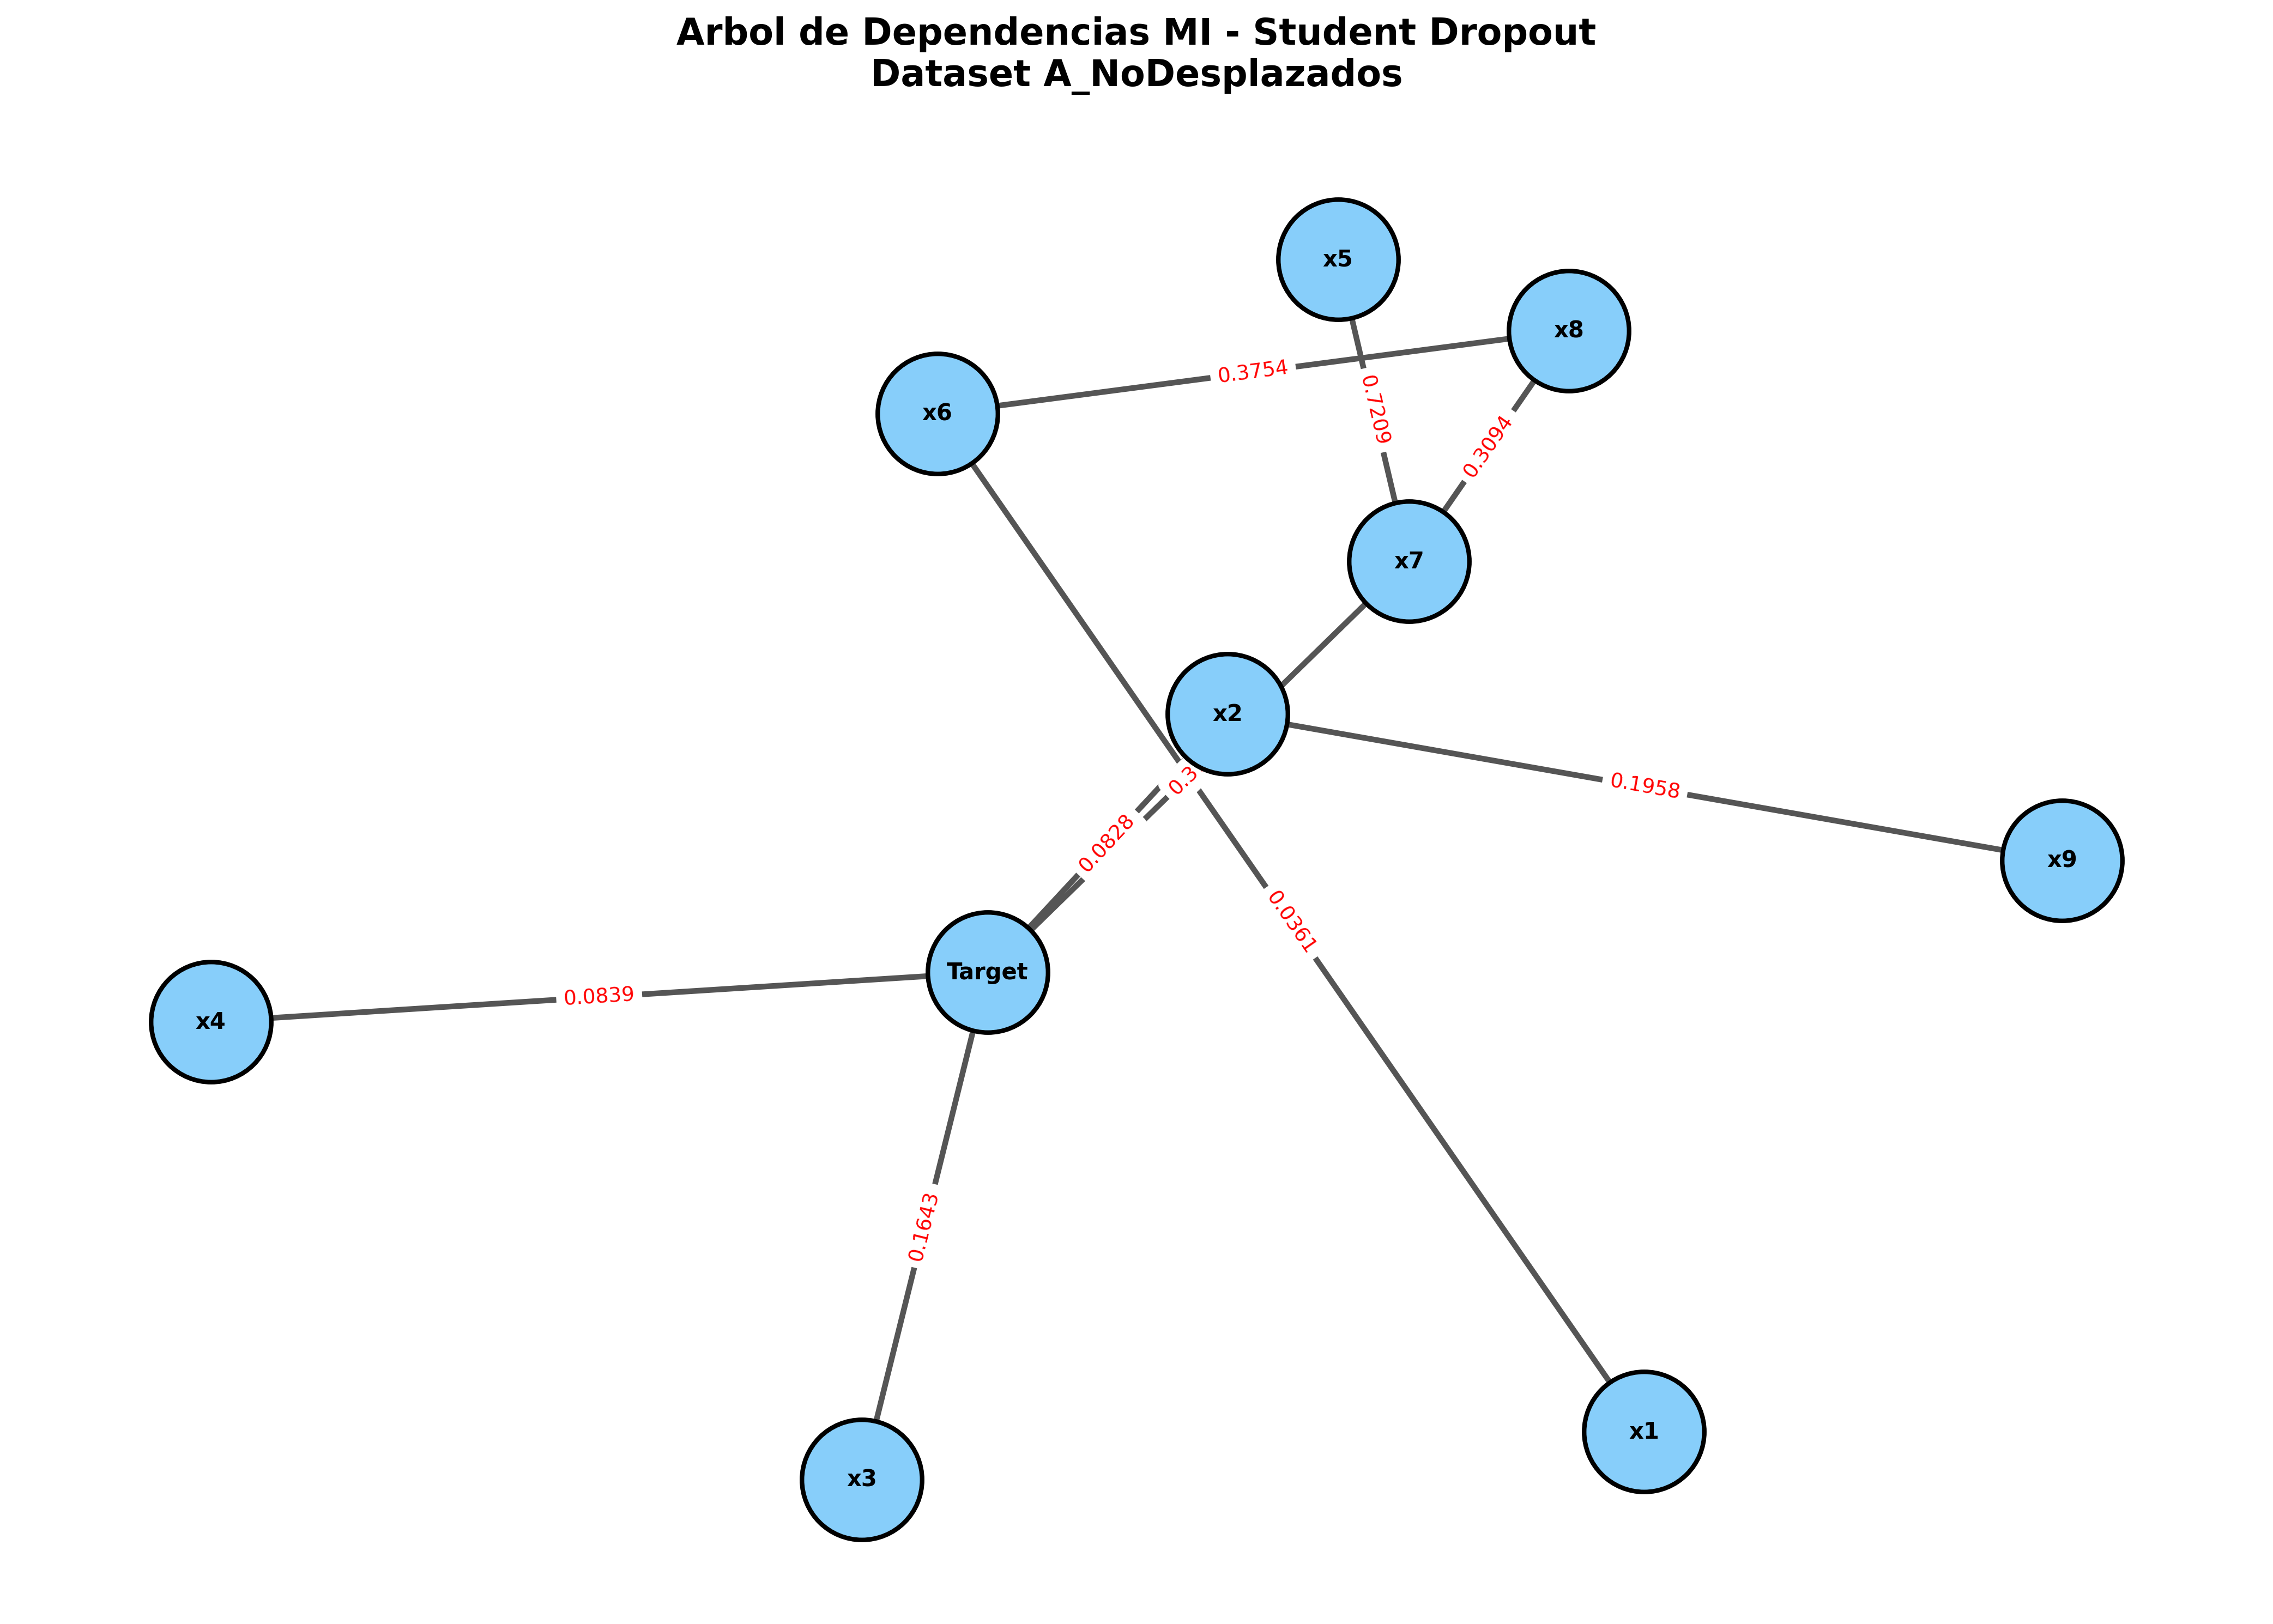
\includegraphics[width=0.85\textwidth]{arbol_A_NoDesplazados.png}
    \caption{Árbol de Expansión Máxima -- Dataset A (No Desplazados).}
    \label{fig:arbolA}
\end{figure}

\begin{figure}[H]
    \centering
    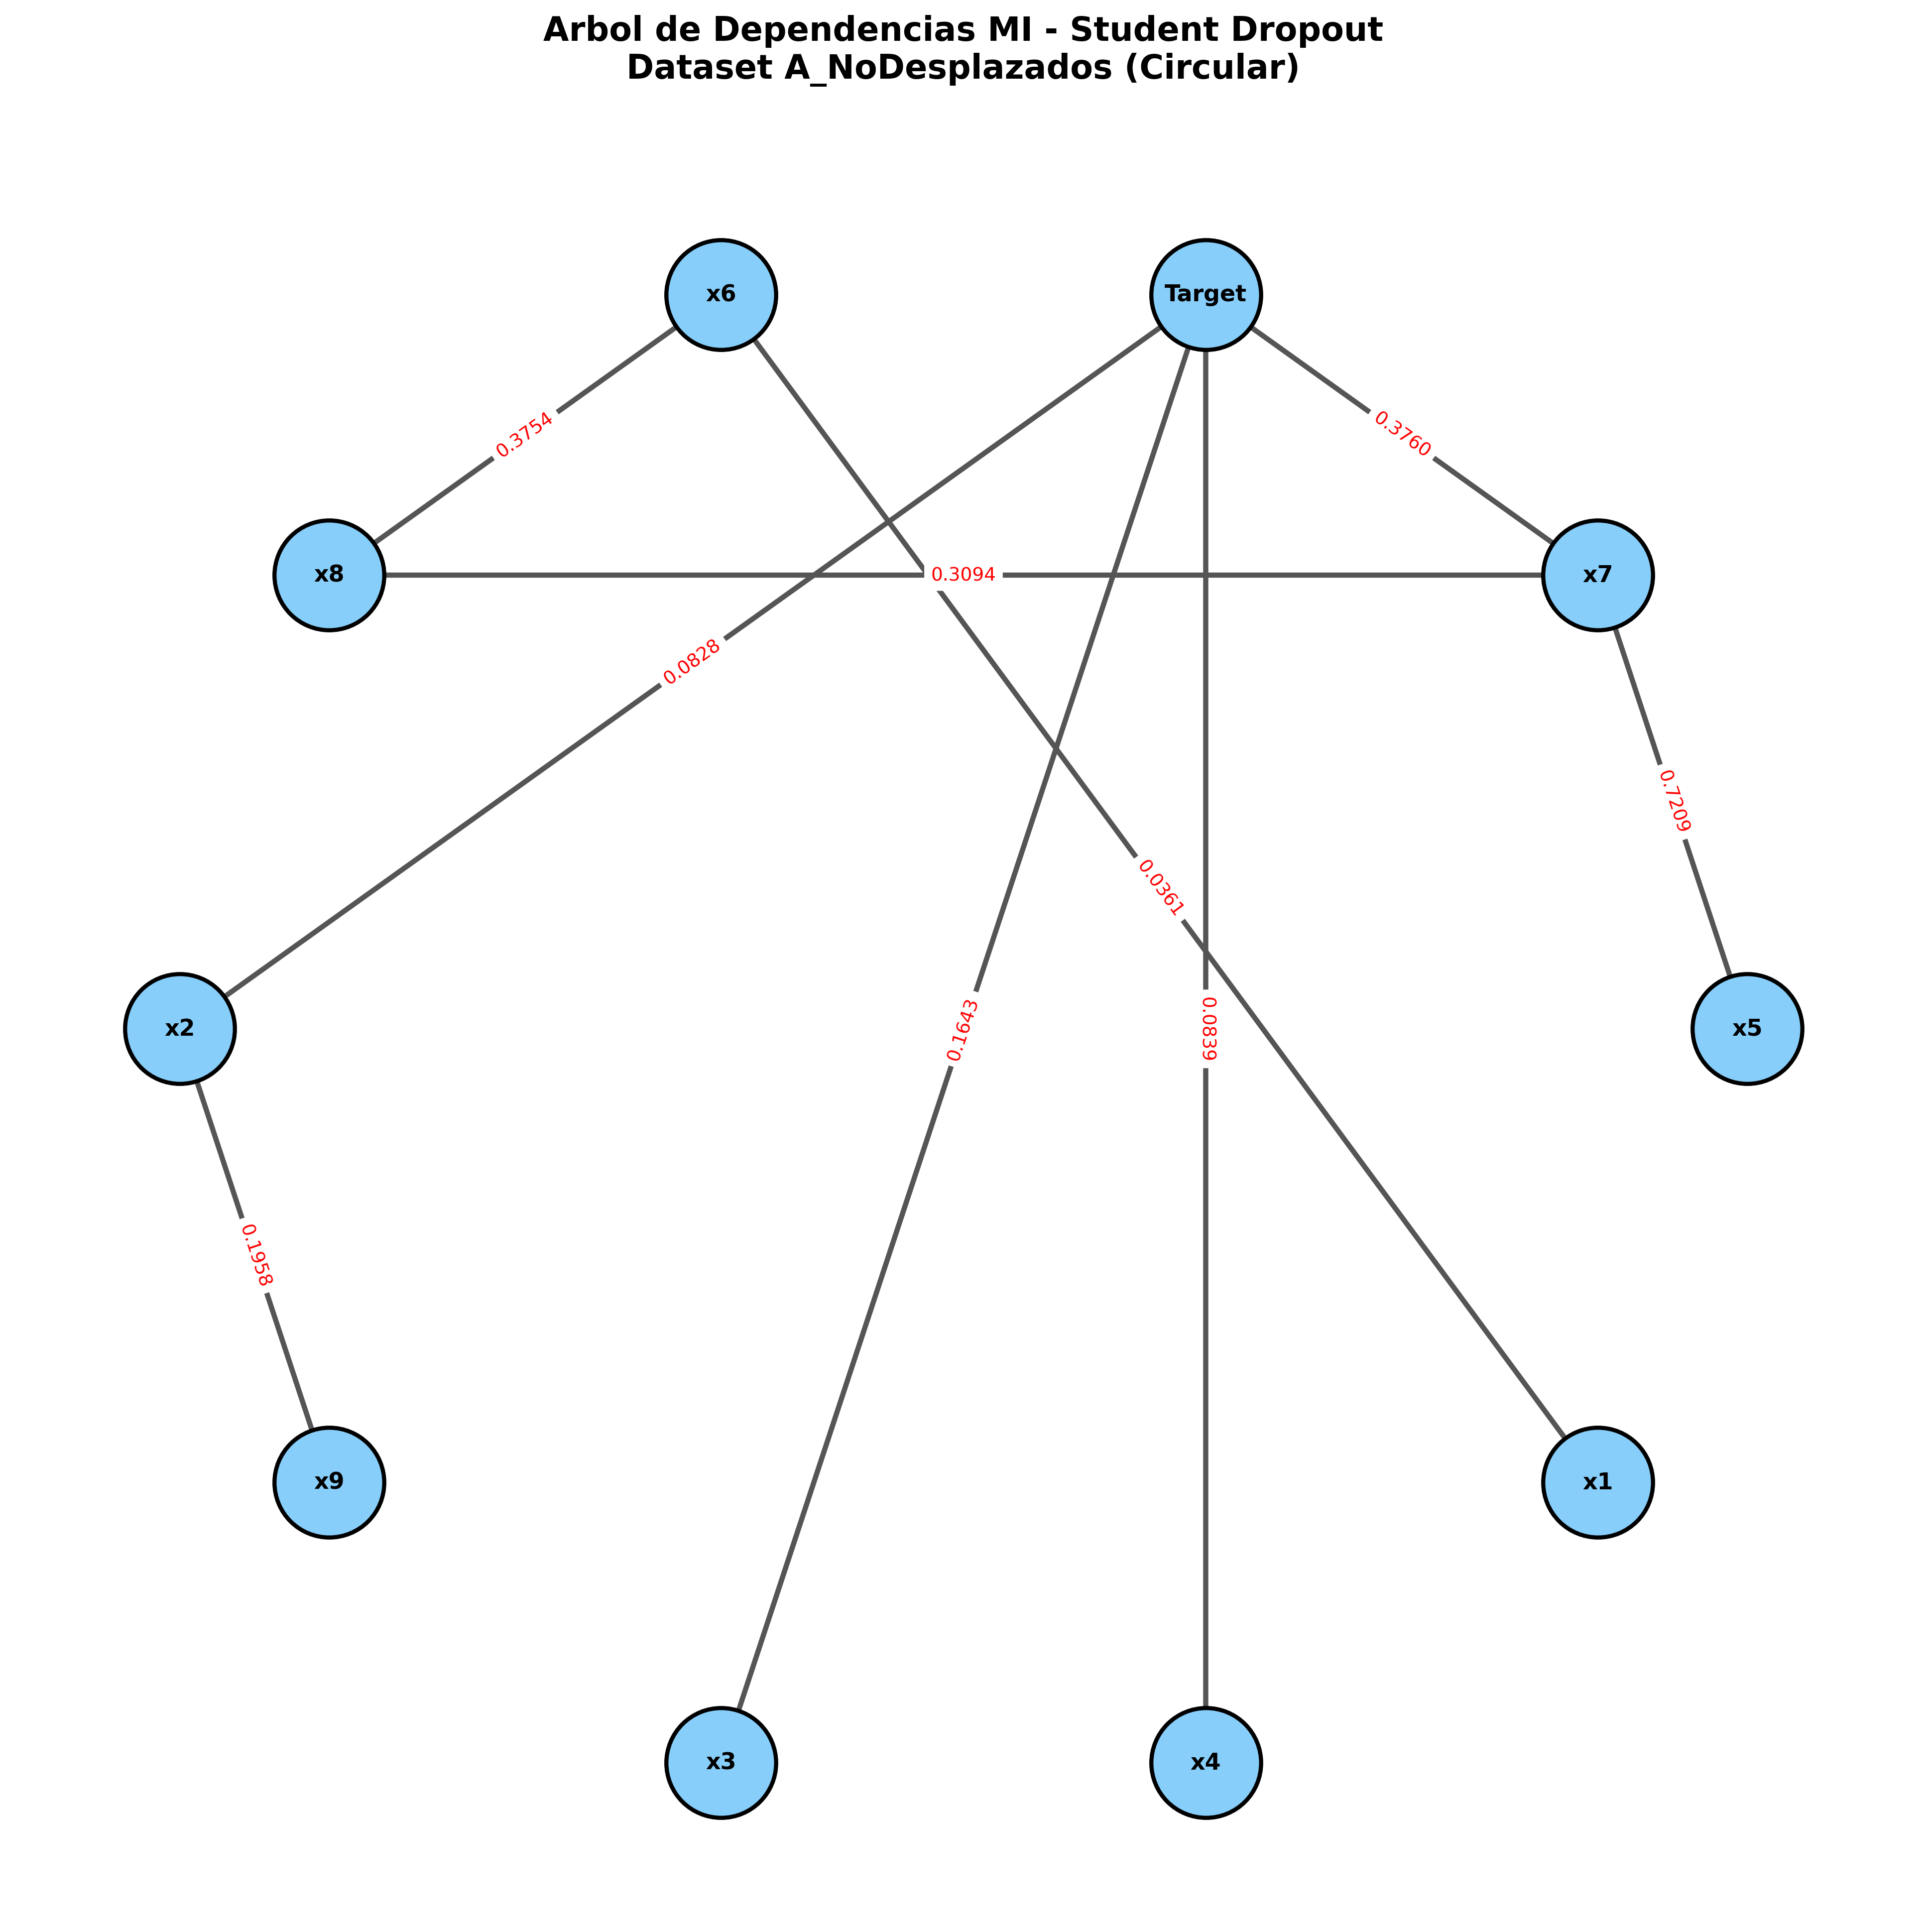
\includegraphics[width=0.75\textwidth]{arbol_A_NoDesplazados_circular.png}
    \caption{Distribución Circular del Árbol -- Dataset A (No Desplazados).}
    \label{fig:arbolA_circ}
\end{figure}

% =============================================
% DATASET B (DESPLAZADOS)
% =============================================
\newpage
\section{Dataset B -- Desplazados (2,426 registros)}

\subsection{Desarrollo de Entropía}

La entropía general es menor en este grupo, reflejando un perfil más homogéneo.


\subsubsection{Calculo para $x1$ (Nota de admision)}
Probabilidades: $p(0) = \frac{743}{2426} = 0.3063$, $p(1) = \frac{900}{2426} = 0.3710$, $p(2) = \frac{783}{2426} = 0.3228$.
\begin{align*}
    H(x1) &= -\big[ (0.3063 \cdot \log_2(0.3063)) + (0.3710 \cdot \log_2(0.3710)) + (0.3228 \cdot \log_2(0.3228)) \big] \\
    H(x1) &= -\big[ (0.3063 \cdot -1.7071) + (0.3710 \cdot -1.4306) + (0.3228 \cdot -1.6315) \big] \\
    H(x1) &= 0.5228 + 0.5307 + 0.5266 = \textbf{1.5801}
\end{align*}

\subsubsection{Calculo para $x2$ (Edad al ingreso)}
Probabilidades: $p(0) = \frac{1355}{2426} = 0.5585$, $p(1) = \frac{703}{2426} = 0.2898$, $p(2) = \frac{368}{2426} = 0.1517$.
\begin{align*}
    H(x2) &= -\big[ (0.5585 \cdot \log_2(0.5585)) + (0.2898 \cdot \log_2(0.2898)) + (0.1517 \cdot \log_2(0.1517)) \big] \\
    H(x2) &= -\big[ (0.5585 \cdot -0.8403) + (0.2898 \cdot -1.7870) + (0.1517 \cdot -2.7208) \big] \\
    H(x2) &= 0.4693 + 0.5178 + 0.4127 = \textbf{1.3999}
\end{align*}

\subsubsection{Calculo para $x3$ (Pagos al dia)}
Probabilidades: $p(0) = \frac{221}{2426} = 0.0911$, $p(1) = \frac{2205}{2426} = 0.9089$.
\begin{align*}
    H(x3) &= -\left[ (0.0911 \cdot \log_2(0.0911)) + (0.9089 \cdot \log_2(0.9089)) \right] \\
    H(x3) &= -\left[ (0.0911 \cdot -3.4565) + (0.9089 \cdot -0.1378) \right] \\
    H(x3) &= 0.3149 + 0.1252 = \textbf{0.4401}
\end{align*}

\subsubsection{Calculo para $x4$ (Becado)}
Probabilidades: $p(0) = \frac{1754}{2426} = 0.7230$, $p(1) = \frac{672}{2426} = 0.2770$.
\begin{align*}
    H(x4) &= -\left[ (0.7230 \cdot \log_2(0.7230)) + (0.2770 \cdot \log_2(0.2770)) \right] \\
    H(x4) &= -\left[ (0.7230 \cdot -0.4679) + (0.2770 \cdot -1.8520) \right] \\
    H(x4) &= 0.3383 + 0.5130 = \textbf{0.8513}
\end{align*}

\subsubsection{Calculo para $x5$ (Aprobados 1er semestre)}
Probabilidades: $p(0) = \frac{851}{2426} = 0.3508$, $p(1) = \frac{1096}{2426} = 0.4518$, $p(2) = \frac{479}{2426} = 0.1974$.
\begin{align*}
    H(x5) &= -\big[ (0.3508 \cdot \log_2(0.3508)) + (0.4518 \cdot \log_2(0.4518)) + (0.1974 \cdot \log_2(0.1974)) \big] \\
    H(x5) &= -\big[ (0.3508 \cdot -1.5113) + (0.4518 \cdot -1.1463) + (0.1974 \cdot -2.3405) \big] \\
    H(x5) &= 0.5302 + 0.5179 + 0.4621 = \textbf{1.5102}
\end{align*}

\subsubsection{Calculo para $x6$ (Nota media 1er semestre)}
Probabilidades: $p(0) = \frac{707}{2426} = 0.2914$, $p(1) = \frac{875}{2426} = 0.3607$, $p(2) = \frac{844}{2426} = 0.3479$.
\begin{align*}
    H(x6) &= -\big[ (0.2914 \cdot \log_2(0.2914)) + (0.3607 \cdot \log_2(0.3607)) + (0.3479 \cdot \log_2(0.3479)) \big] \\
    H(x6) &= -\big[ (0.2914 \cdot -1.7788) + (0.3607 \cdot -1.4712) + (0.3479 \cdot -1.5233) \big] \\
    H(x6) &= 0.5184 + 0.5306 + 0.5299 = \textbf{1.5790}
\end{align*}

\subsubsection{Calculo para $x7$ (Aprobados 2do semestre)}
Probabilidades: $p(0) = \frac{947}{2426} = 0.3904$, $p(1) = \frac{980}{2426} = 0.4040$, $p(2) = \frac{499}{2426} = 0.2057$.
\begin{align*}
    H(x7) &= -\big[ (0.3904 \cdot \log_2(0.3904)) + (0.4040 \cdot \log_2(0.4040)) + (0.2057 \cdot \log_2(0.2057)) \big] \\
    H(x7) &= -\big[ (0.3904 \cdot -1.3571) + (0.4040 \cdot -1.3077) + (0.2057 \cdot -2.2815) \big] \\
    H(x7) &= 0.5298 + 0.5283 + 0.4693 = \textbf{1.5273}
\end{align*}

\subsubsection{Calculo para $x8$ (Nota media 2do semestre)}
Probabilidades: $p(0) = \frac{739}{2426} = 0.3046$, $p(1) = \frac{882}{2426} = 0.3636$, $p(2) = \frac{805}{2426} = 0.3318$.
\begin{align*}
    H(x8) &= -\big[ (0.3046 \cdot \log_2(0.3046)) + (0.3636 \cdot \log_2(0.3636)) + (0.3318 \cdot \log_2(0.3318)) \big] \\
    H(x8) &= -\big[ (0.3046 \cdot -1.7149) + (0.3636 \cdot -1.4597) + (0.3318 \cdot -1.5915) \big] \\
    H(x8) &= 0.5224 + 0.5307 + 0.5281 = \textbf{1.5812}
\end{align*}

\subsubsection{Calculo para $x9$ (Estado civil)}
Probabilidades: $p(0) = \frac{2342}{2426} = 0.9654$, $p(1) = \frac{84}{2426} = 0.0346$.
\begin{align*}
    H(x9) &= -\left[ (0.9654 \cdot \log_2(0.9654)) + (0.0346 \cdot \log_2(0.0346)) \right] \\
    H(x9) &= -\left[ (0.9654 \cdot -0.0508) + (0.0346 \cdot -4.8520) \right] \\
    H(x9) &= 0.0491 + 0.1680 = \textbf{0.2171}
\end{align*}

\subsubsection{Calculo para $Target$ (Target)}
Probabilidades: $p(0) = \frac{669}{2426} = 0.2758$, $p(1) = \frac{433}{2426} = 0.1785$, $p(2) = \frac{1324}{2426} = 0.5458$.
\begin{align*}
    H(Target) &= -\big[ (0.2758 \cdot \log_2(0.2758)) + (0.1785 \cdot \log_2(0.1785)) + (0.5458 \cdot \log_2(0.5458)) \big] \\
    H(Target) &= -\big[ (0.2758 \cdot -1.8585) + (0.1785 \cdot -2.4861) + (0.5458 \cdot -0.8737) \big] \\
    H(Target) &= 0.5125 + 0.4437 + 0.4768 = \textbf{1.4331}
\end{align*}

\subsection{Matriz de Información Mutua}

\subsubsection{Ejemplo detallado: $x_5$ con $x_7$}
Probabilidades conjuntas principales y sus términos:

\begin{align*}
    \text{Term. } (0,0) &= 0.3199 \cdot \log_2\left(\frac{0.3199}{0.3821 \cdot 0.3904}\right) = 0.3199 \cdot \log_2(2.1458) = \mathbf{+0.3521} \\
    \text{Term. } (1,1) &= 0.3293 \cdot \log_2\left(\frac{0.3293}{0.4398 \cdot 0.4040}\right) = 0.3293 \cdot \log_2(1.8530) = \mathbf{+0.2929} \\
    \text{Term. } (2,2) &= 0.1311 \cdot \log_2\left(\frac{0.1311}{0.1781 \cdot 0.2057}\right) = 0.1311 \cdot \log_2(3.5808) = \mathbf{+0.2406}
\end{align*}
\textbf{Suma Total:} $IM(x_5, x_7) = \textbf{0.8335}$ (incluyendo términos cruzados negativos)

\subsubsection{Matriz Resultante (10$\times$10)}

\begin{table}[H]
    \centering
    \footnotesize
    \begin{tabular}{c|cccccccccc}
        \toprule
        & $\mathbf{x_1}$ & $\mathbf{x_2}$ & $\mathbf{x_3}$ & $\mathbf{x_4}$ & $\mathbf{x_5}$ & $\mathbf{x_6}$ & $\mathbf{x_7}$ & $\mathbf{x_8}$ & $\mathbf{x_9}$ & \textbf{Target} \\
        \midrule
        $\mathbf{x_1}$ & 0 & 0.0305 & 0.0061 & 0.0037 & 0.0116 & 0.0307 & 0.0139 & 0.0231 & 0.0028 & 0.0106 \\
        $\mathbf{x_2}$ & 0.0305 & 0 & 0.0158 & 0.0277 & 0.0261 & 0.0231 & 0.0251 & 0.0213 & 0.0782 & 0.0467 \\
        $\mathbf{x_3}$ & 0.0061 & 0.0158 & 0 & 0.0121 & 0.0356 & 0.0312 & 0.0491 & 0.0451 & 0.0002 & 0.0992 \\
        $\mathbf{x_4}$ & 0.0037 & 0.0277 & 0.0121 & 0 & 0.0347 & 0.0263 & 0.0482 & 0.0255 & 0.0070 & 0.0585 \\
        $\mathbf{x_5}$ & 0.0116 & 0.0261 & 0.0356 & 0.0347 & 0 & 0.2954 & \textbf{0.8335} & 0.3204 & 0.0062 & 0.2331 \\
        $\mathbf{x_6}$ & 0.0307 & 0.0231 & 0.0312 & 0.0263 & 0.2954 & 0 & 0.2955 & \textbf{0.4695} & 0.0068 & 0.1562 \\
        $\mathbf{x_7}$ & 0.0139 & 0.0251 & 0.0491 & 0.0482 & \textbf{0.8335} & 0.2955 & 0 & 0.3632 & 0.0049 & 0.2964 \\
        $\mathbf{x_8}$ & 0.0231 & 0.0213 & 0.0451 & 0.0255 & 0.3204 & \textbf{0.4695} & 0.3632 & 0 & 0.0052 & 0.2226 \\
        $\mathbf{x_9}$ & 0.0028 & \textbf{0.0782} & 0.0002 & 0.0070 & 0.0062 & 0.0068 & 0.0049 & 0.0052 & 0 & 0.0071 \\
        \textbf{Target} & 0.0106 & 0.0467 & 0.0992 & 0.0585 & 0.2331 & 0.1562 & \textbf{0.2964} & 0.2226 & 0.0071 & 0 \\
        \bottomrule
    \end{tabular}
    \caption{Matriz de Información Mutua -- Dataset B.}
\end{table}

\subsection{Algoritmo de Kruskal (MST)}

\begin{enumerate}[label=\textbf{\arabic*.}]
    \item $x_5 - x_7$ (Peso: 0.8335) $\rightarrow$ \textbf{Aceptado}
    \item $x_6 - x_8$ (Peso: 0.4695) $\rightarrow$ \textbf{Aceptado}
    \item $x_7 - x_8$ (Peso: 0.3632) $\rightarrow$ \textbf{Aceptado}
    \item $x_6 - x_5$ (Peso: 0.2954) $\rightarrow$ \textbf{Rechazado} (Ciclo con $x_5$, $x_7$, $x_8$)
    \item $x_7 - Target$ (Peso: 0.2964) $\rightarrow$ \textbf{Aceptado}
    \item $x_2 - x_9$ (Peso: 0.0782) $\rightarrow$ \textbf{Aceptado}
    \item $x_3 - Target$ (Peso: 0.0992) $\rightarrow$ \textbf{Aceptado}
    \item $x_4 - Target$ (Peso: 0.0585) $\rightarrow$ \textbf{Aceptado}
    \item $x_2 - Target$ (Peso: 0.0467) $\rightarrow$ \textbf{Aceptado}
    \item $x_1 - x_6$ (Peso: 0.0307) $\rightarrow$ \textbf{Aceptado} (Última arista)
\end{enumerate}

\textbf{Cálculo del Peso del MST (Dataset B):}
\begin{equation}
    MST_B = 0.8335 + 0.4695 + 0.3632 + 0.2964 + 0.0782 + 0.0992 + 0.0585 + 0.0467 + 0.0307 = \textbf{2.2759}
\end{equation}

\subsection{Validación por Algoritmo de Prim}
Partiendo del nodo Target:

\begin{itemize}
    \item \textbf{Paso 1:} Desde Target $\rightarrow$ Mayor: \textbf{$x_7$} (0.2964).
    \item \textbf{Paso 2:} Desde $x_7$ $\rightarrow$ Mayor: \textbf{$x_5$} (0.8335).
    \item \textbf{Paso 3:} Desde $x_7$ $\rightarrow$ Mayor libre: \textbf{$x_8$} (0.3632).
    \item \textbf{Paso 4:} Desde $x_8$ $\rightarrow$ Mayor: \textbf{$x_6$} (0.4695).
    \item \textbf{Paso 5:} Desde Target $\rightarrow$ Mayor libre: \textbf{$x_3$} (0.0992).
    \item \textbf{Paso 6:} Desde Target $\rightarrow$ Mayor libre: \textbf{$x_4$} (0.0585).
    \item \textbf{Paso 7:} Desde Target $\rightarrow$ Mayor libre: \textbf{$x_2$} (0.0467).
    \item \textbf{Paso 8:} Desde $x_2$ $\rightarrow$ Mayor libre: \textbf{$x_9$} (0.0782).
    \item \textbf{Paso 9:} Desde $x_6$ $\rightarrow$ Mayor libre: \textbf{$x_1$} (0.0307).
\end{itemize}

Prim genera las mismas 9 aristas, confirmando un MST de peso \textbf{2.2759}.

\subsection{Árbol de Dependencias}

\begin{figure}[H]
    \centering
    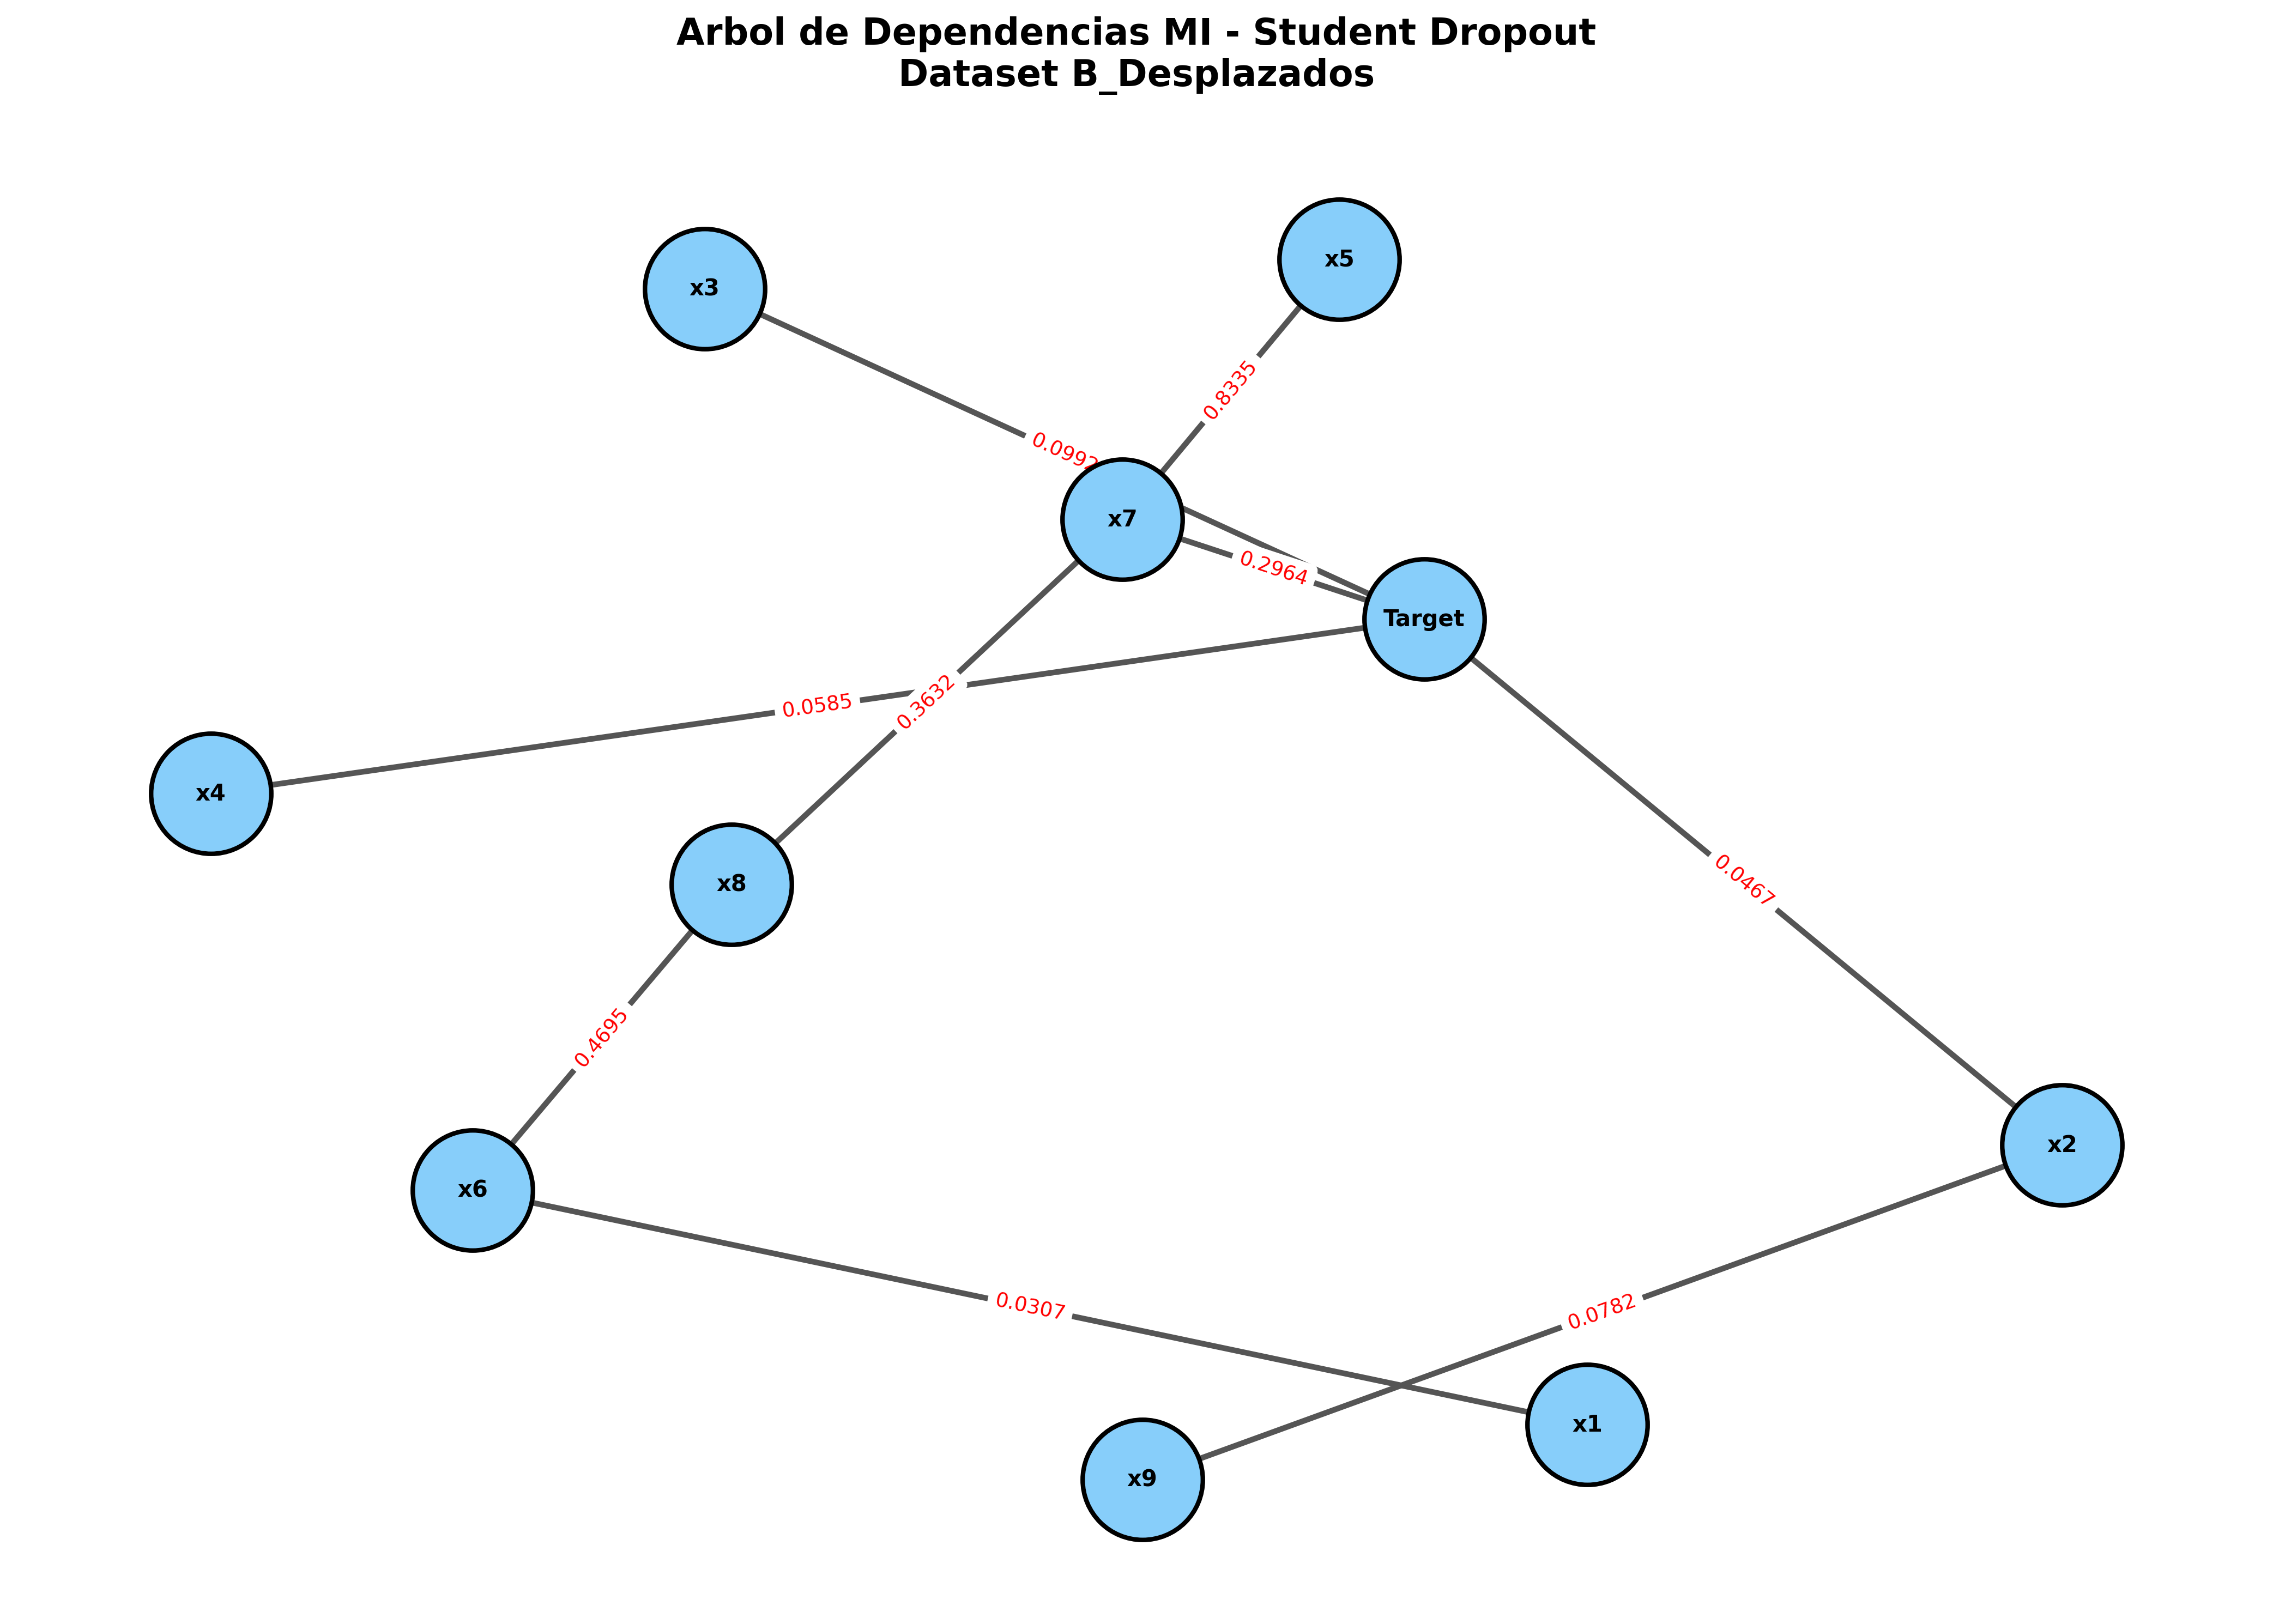
\includegraphics[width=0.85\textwidth]{arbol_B_Desplazados.png}
    \caption{Árbol de Expansión Máxima -- Dataset B (Desplazados).}
    \label{fig:arbolB}
\end{figure}

\begin{figure}[H]
    \centering
    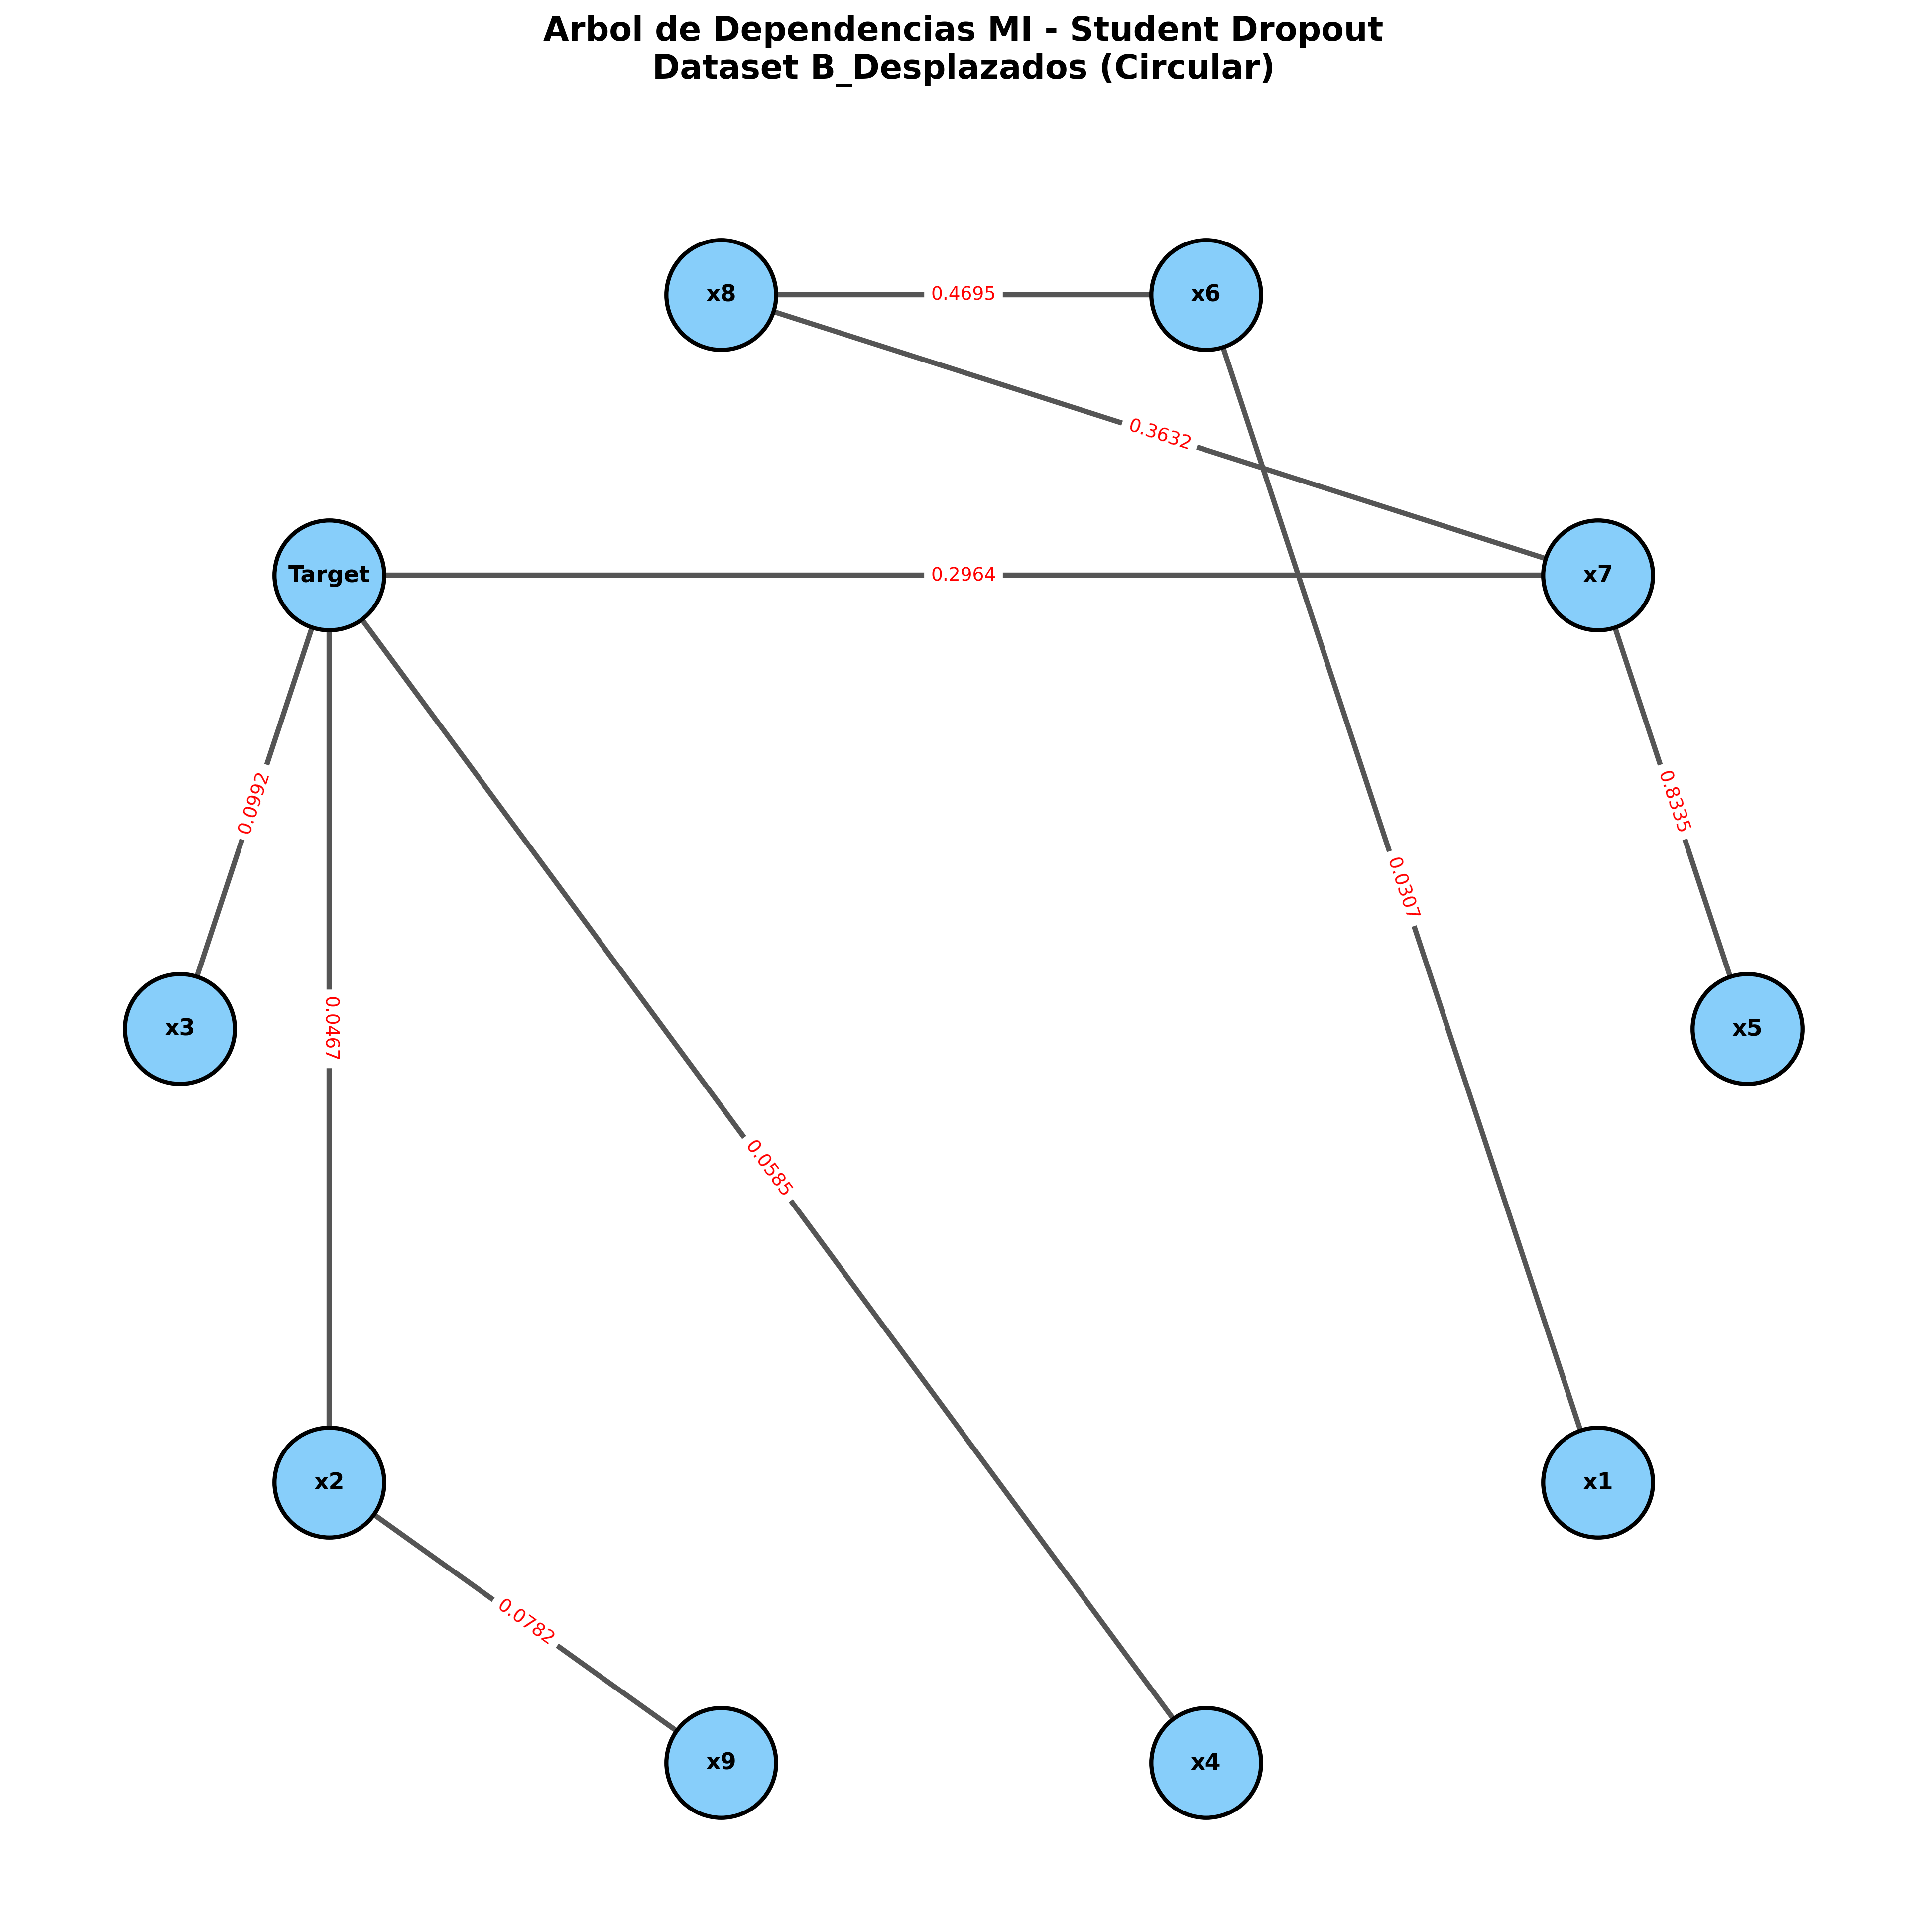
\includegraphics[width=0.75\textwidth]{arbol_B_Desplazados_circular.png}
    \caption{Distribución Circular del Árbol -- Dataset B (Desplazados).}
    \label{fig:arbolB_circ}
\end{figure}

% =============================================
% COMPARATIVA Y ANÁLISIS
% =============================================
\newpage
\section{Análisis Comparativo}

\subsection{Comparativa de Entropías}

\begin{table}[H]
    \centering
    \begin{tabular}{c|ccc}
        \toprule
        \textbf{Variable} & $H(A)$ & $H(B)$ & $H(Original)$ \\
        \midrule
        $x_1$ (Nota admisión) & 1.5773 & 1.5801 & 1.5850 \\
        $x_2$ (Edad) & 1.4795 & 1.3999 & 1.5435 \\
        $x_3$ (Pagos al día) & 0.6189 & 0.4401 & 0.5275 \\
        $x_4$ (Becado) & 0.7485 & 0.8513 & 0.8088 \\
        $x_5$ (1sem aprobados) & 1.4897 & 1.5102 & 1.5055 \\
        $x_6$ (1sem nota) & 1.5724 & 1.5790 & 1.5840 \\
        $x_7$ (2sem aprobados) & 1.4851 & 1.5273 & 1.5126 \\
        $x_8$ (2sem nota) & 1.5754 & 1.5812 & 1.5824 \\
        $x_9$ (Estado civil) & 0.7428 & 0.2171 & 0.5123 \\
        \midrule
        Target & 1.4970 & 1.4331 & 1.4713 \\
        \bottomrule
    \end{tabular}
    \caption{Comparativa de entropías entre datasets.}
\end{table}

\textbf{Observación sobre $x_9$ (Estado civil):} En el dataset original, el estado civil tiene una entropía moderada ($H = 0.5123$) con distribución $88.6\%$ solteros y $11.4\%$ otros. Al particionar por desplazamiento, el Dataset A presenta $H_A = 0.7428$, mientras que el Dataset B colapsa a $H_B = 0.2171$. Esto evidencia que los estudiantes desplazados son casi en su totalidad solteros ($92.9\%$), mientras que los no desplazados tienen mayor diversidad de estados civiles.

\subsection{Comparativa de Árboles MST}

\begin{table}[H]
    \centering
    \begin{tabular}{c|c|c}
        \toprule
        & \textbf{Dataset A (No Desp)} & \textbf{Dataset B (Desp)} \\
        \midrule
        Arista 1 & $x_5 - x_7$ (0.7209) & $x_5 - x_7$ (0.8335) \\
        Arista 2 & $x_6 - x_8$ (0.3754) & $x_6 - x_8$ (0.4695) \\
        Arista 3 & $x_7 - Target$ (0.3760) & $x_7 - x_8$ (0.3632) \\
        Arista 4 & $x_7 - x_8$ (0.3094) & $x_7 - Target$ (0.2964) \\
        Arista 5 & $x_2 - x_9$ (0.1958) & $x_2 - x_9$ (0.0782) \\
        Arista 6 & $x_3 - Target$ (0.1643) & $x_3 - Target$ (0.0992) \\
        Arista 7 & $x_4 - Target$ (0.0839) & $x_4 - Target$ (0.0585) \\
        Arista 8 & $x_2 - Target$ (0.0828) & $x_2 - Target$ (0.0467) \\
        Arista 9 & $x_1 - x_6$ (0.0336) & $x_1 - x_6$ (0.0307) \\
        \midrule
        \rowcolor{blue!15}
        Peso total & \textbf{2.3421} & \textbf{2.2759} \\
        \bottomrule
    \end{tabular}
    \caption{Comparativa de aristas del MST.}
\end{table}

\textbf{Hallazgos principales:}
\begin{itemize}
    \item Ambos datasets conservan una estructura muy similar: el \textbf{bloque académico} ($x_5$, $x_6$, $x_7$, $x_8$) forma el núcleo del árbol, con $x_7$ (2do semestre aprobados) como puente hacia el Target.
    \item La conexión $x_5 - x_7$ es consistentemente la de mayor peso en ambos datasets (0.7209 en A, 0.8335 en B), indicando una fuerte dependencia entre el rendimiento del primer y segundo semestre.
    \item El Target se conecta directamente a 4 variables en ambos datasets: $x_7$ (rendimiento), $x_3$ (pagos), $x_4$ (beca) y $x_2$ (edad), siendo $x_7$ el predictor más fuerte.
    \item Los pesos totales del MST son muy similares (2.3421 vs 2.2759), indicando que la estructura global de dependencias es robusta a la partición por desplazamiento.
    \item $x_1$ (nota de admisión) es consistentemente la variable más periférica, conectada a $x_6$ con pesos bajos en ambos datasets.
\end{itemize}

% =============================================
% ANÁLISIS DE SENSIBILIDAD — rVP
% =============================================
\newpage
\section{Análisis de Sensibilidad -- Método rVP}

\subsection{Matriz de Distancias de Camino}

La distancia de camino $d(x_i, x_j)$ se define como la suma de los pesos de todas las aristas que conforman el camino único entre dos nodos en el MST:

\begin{equation}
    d(x_i, x_j) = \sum_{e \in \text{camino}(x_i \rightarrow x_j)} w(e)
\end{equation}

\subsubsection{Dataset A (No Desplazados)}

\begin{table}[H]
    \centering
    \footnotesize
    \begin{tabular}{c|cccccccccc|c}
        \toprule
        $d(i,j)$ & $\mathbf{x_1}$ & $\mathbf{x_2}$ & $\mathbf{x_3}$ & $\mathbf{x_4}$ & $\mathbf{x_5}$ & $\mathbf{x_6}$ & $\mathbf{x_7}$ & $\mathbf{x_8}$ & $\mathbf{x_9}$ & \textbf{Target} & $\mathbf{\Sigma}$ \\
        \midrule
        $\mathbf{x_1}$   & 0 & 0.4876 & 0.5739 & 0.4935 & 0.7545 & 0.0336 & 0.3786 & 0.3430 & 0.5980 & 0.4424 & 4.1052 \\
        $\mathbf{x_2}$   & 0.4876 & 0 & 0.2471 & 0.1667 & 0.3417 & 0.4540 & 0.0539 & 0.3633 & 0.1958 & 0.0828 & 2.3929 \\
        $\mathbf{x_3}$   & 0.5739 & 0.2471 & 0 & 0.2485 & 0.5525 & 0.5403 & 0.1643 & 0.4737 & 0.4429 & 0.1643 & 3.4074 \\
        $\mathbf{x_4}$   & 0.4935 & 0.1667 & 0.2485 & 0 & 0.4669 & 0.4599 & 0.0839 & 0.3932 & 0.3625 & 0.0839 & 2.7589 \\
        $\mathbf{x_5}$   & 0.7545 & 0.3417 & 0.5525 & 0.4669 & 0 & 0.7545 & 0.7209 & 0.3094 & 0.5375 & 0.3760 & 4.8129 \\
        $\mathbf{x_6}$   & 0.0336 & 0.4540 & 0.5403 & 0.4599 & 0.7545 & 0 & 0.3754 & 0.3754 & 0.5644 & 0.4088 & 3.9660 \\
        $\mathbf{x_7}$   & 0.3786 & 0.0539 & 0.1643 & 0.0839 & 0.7209 & 0.3754 & 0 & 0.3094 & 0.2497 & 0.3760 & 2.7120 \\
        $\mathbf{x_8}$   & 0.3430 & 0.3633 & 0.4737 & 0.3932 & 0.3094 & 0.3754 & 0.3094 & 0 & 0.4737 & 0.6854 & 3.7264 \\
        $\mathbf{x_9}$   & 0.5980 & 0.1958 & 0.4429 & 0.3625 & 0.5375 & 0.5644 & 0.2497 & 0.4737 & 0 & 0.2786 & 3.7030 \\
        \textbf{Target}  & 0.4424 & 0.0828 & 0.1643 & 0.0839 & 0.3760 & 0.4088 & 0.3760 & 0.6854 & 0.2786 & 0 & 2.8981 \\
        \bottomrule
    \end{tabular}
    \caption{Matriz de distancias de caminos -- Dataset A.}
\end{table}

\subsubsection{Dataset B (Desplazados)}

\begin{table}[H]
    \centering
    \footnotesize
    \begin{tabular}{c|cccccccccc|c}
        \toprule
        $d(i,j)$ & $\mathbf{x_1}$ & $\mathbf{x_2}$ & $\mathbf{x_3}$ & $\mathbf{x_4}$ & $\mathbf{x_5}$ & $\mathbf{x_6}$ & $\mathbf{x_7}$ & $\mathbf{x_8}$ & $\mathbf{x_9}$ & \textbf{Target} & $\mathbf{\Sigma}$ \\
        \midrule
        $\mathbf{x_1}$   & 0 & 0.3558 & 0.4754 & 0.4640 & 0.8642 & 0.0307 & 0.3936 & 0.3937 & 0.3990 & 0.4051 & 3.7817 \\
        $\mathbf{x_2}$   & 0.3558 & 0 & 0.1459 & 0.1052 & 0.3542 & 0.3252 & 0.0625 & 0.2945 & 0.0782 & 0.0467 & 1.7682 \\
        $\mathbf{x_3}$   & 0.4754 & 0.1459 & 0 & 0.1577 & 0.4888 & 0.4455 & 0.0992 & 0.4632 & 0.2241 & 0.0992 & 2.5988 \\
        $\mathbf{x_4}$   & 0.4640 & 0.1052 & 0.1577 & 0 & 0.4442 & 0.4339 & 0.0585 & 0.4217 & 0.1834 & 0.0585 & 2.3270 \\
        $\mathbf{x_5}$   & 0.8642 & 0.3542 & 0.4888 & 0.4442 & 0 & 0.8329 & 0.8335 & 0.3632 & 0.3974 & 0.2964 & 4.8748 \\
        $\mathbf{x_6}$   & 0.0307 & 0.3252 & 0.4455 & 0.4339 & 0.8329 & 0 & 0.4695 & 0.4695 & 0.3684 & 0.3758 & 3.7515 \\
        $\mathbf{x_7}$   & 0.3936 & 0.0625 & 0.0992 & 0.0585 & 0.8335 & 0.4695 & 0 & 0.3632 & 0.1407 & 0.2964 & 2.7172 \\
        $\mathbf{x_8}$   & 0.3937 & 0.2945 & 0.4632 & 0.4217 & 0.3632 & 0.4695 & 0.3632 & 0 & 0.3377 & 0.6596 & 3.7665 \\
        $\mathbf{x_9}$   & 0.3990 & 0.0782 & 0.2241 & 0.1834 & 0.3974 & 0.3684 & 0.1407 & 0.3377 & 0 & 0.1249 & 2.2538 \\
        \textbf{Target}  & 0.4051 & 0.0467 & 0.0992 & 0.0585 & 0.2964 & 0.3758 & 0.2964 & 0.6596 & 0.1249 & 0 & 2.3627 \\
        \bottomrule
    \end{tabular}
    \caption{Matriz de distancias de caminos -- Dataset B.}
\end{table}

\subsection{Análisis Diferencial ($\Delta = \Sigma_A - \Sigma_B$)}

\begin{table}[H]
    \centering
    \begin{tabular}{c|ccc|c|c}
        \toprule
        \textbf{Variable} & $\mathbf{\Sigma_A}$ & $\mathbf{\Sigma_B}$ & $\mathbf{\Delta}$ & $\mathbf{|\Delta|}$ & \textbf{¿Crítica?} \\
        \midrule
        $x_1$ (Nota admisión) & 4.1052 & 3.7817 & +0.3235 & 0.3235 & No \\
        $x_2$ (Edad) & 2.3929 & 1.7682 & +0.6247 & 0.6247 & \textbf{Sí} \\
        $x_3$ (Pagos al día) & 3.4074 & 2.5988 & +0.8086 & 0.8086 & \textbf{Sí} \\
        $x_4$ (Becado) & 2.7589 & 2.3270 & +0.4319 & 0.4319 & No \\
        $x_5$ (1sem aprobados) & 4.8129 & 4.8748 & -0.0619 & 0.0619 & No \\
        $x_6$ (1sem nota) & 3.9660 & 3.7515 & +0.2145 & 0.2145 & No \\
        $x_7$ (2sem aprobados) & 2.7120 & 2.7172 & -0.0052 & 0.0052 & No \\
        $x_8$ (2sem nota) & 3.7264 & 3.7665 & -0.0401 & 0.0401 & No \\
        \rowcolor{red!20}
        $x_9$ (Estado civil) & 3.7030 & 2.2538 & \textbf{+1.4492} & 1.4492 & \textbf{Sí} \\
        Target & 2.8981 & 2.3627 & +0.5354 & 0.5354 & \textbf{Sí} \\
        \bottomrule
    \end{tabular}
    \caption{Análisis diferencial rVP (umbral: $|\Delta| > 0.5$).}
\end{table}

\subsection{Variables Críticas}

Con un umbral de $|\Delta| > 0.5$, se identifican 4 variables críticas:

\begin{enumerate}
    \item \textbf{$x_9$ (Estado civil, $\Delta = +1.4492$)}: Es la variable más afectada por la partición. En el Dataset B (desplazados), $x_9$ tiene una entropía mínima ($H_B = 0.2171$) porque el $92.9\%$ de los estudiantes desplazados son solteros. Esto la acerca al centro del árbol en B ($\Sigma_B = 2.25$), mientras que en A está más en la periferia ($\Sigma_A = 3.70$).

    \item \textbf{$x_3$ (Pagos al día, $\Delta = +0.8086$)}: En el Dataset A (no desplazados), $x_3$ está más alejado del centro ($\Sigma_A = 3.41$), mientras que en B se acerca ($\Sigma_B = 2.60$). Esto sugiere que la situación financiera (pagos al día) es más relevante estructuralmente en los estudiantes desplazados.

    \item \textbf{$x_2$ (Edad, $\Delta = +0.6247$)}: Su centralidad varía entre grupos. En B está más cerca del centro ($\Sigma_B = 1.77$), actuando como puente entre $x_9$ y Target, mientras que en A está algo más alejada ($\Sigma_A = 2.39$).

    \item \textbf{Target ($\Delta = +0.5354$)}: La variable objetivo también cambia su posición topológica, estando más integrada al árbol en el Dataset B ($\Sigma_B = 2.36$) que en el A ($\Sigma_A = 2.90$).
\end{enumerate}

\subsection{Conclusiones del Análisis de Sensibilidad}

\begin{itemize}
    \item El \textbf{bloque académico} ($x_5$, $x_6$, $x_7$, $x_8$) muestra una \textbf{robustez estructural notable}: ninguna de estas variables es crítica, indicando que las relaciones de rendimiento académico son estables independientemente del desplazamiento.

    \item \textbf{$x_9$ (estado civil)} emerge como la variable más crítica ($\Delta = +1.4492$). La partición por desplazamiento separa casi perfectamente a los solteros (grupo B) del resto (grupo A), alterando completamente su rol topológico.

    \item Desde la perspectiva del método rVP, la partición por desplazamiento \textbf{afecta principalmente a variables socio-demográficas} ($x_9$, $x_2$) y financieras ($x_3$), mientras que \textbf{el núcleo académico permanece inalterado}. Esto valida que el rendimiento académico es un predictor robusto del abandono universitario, independientemente de la condición de desplazamiento.
\end{itemize}

% =============================================
% REDES BAYESIANAS
% =============================================
\newpage
\section{Redes Bayesianas -- Algoritmo de Chow-Liu}

El árbol de dependencias construido mediante Información Mutua y el algoritmo de Kruskal es, de hecho, el resultado del \textbf{algoritmo de Chow-Liu} para el aprendizaje de la estructura de una red Bayesiana. Chow-Liu (1968) demostró que la estructura de árbol que maximiza la verosimilitud de los datos es exactamente el Árbol de Expansión de Peso Máximo calculado sobre la matriz de Información Mutua. En otras palabras, el MST obtenido en las secciones anteriores es la \textbf{estructura óptima de red Bayesiana tipo árbol} para este dataset.

\subsection{Construcción del DAG}

Para convertir el MST (grafo no dirigido) en una red Bayesiana (grafo dirigido acíclico, DAG), se selecciona el nodo \texttt{Target} como raíz y se orientan todas las aristas alejándose de él mediante un recorrido en anchura (BFS). El resultado es el siguiente DAG:

\begin{figure}[H]
    \centering
    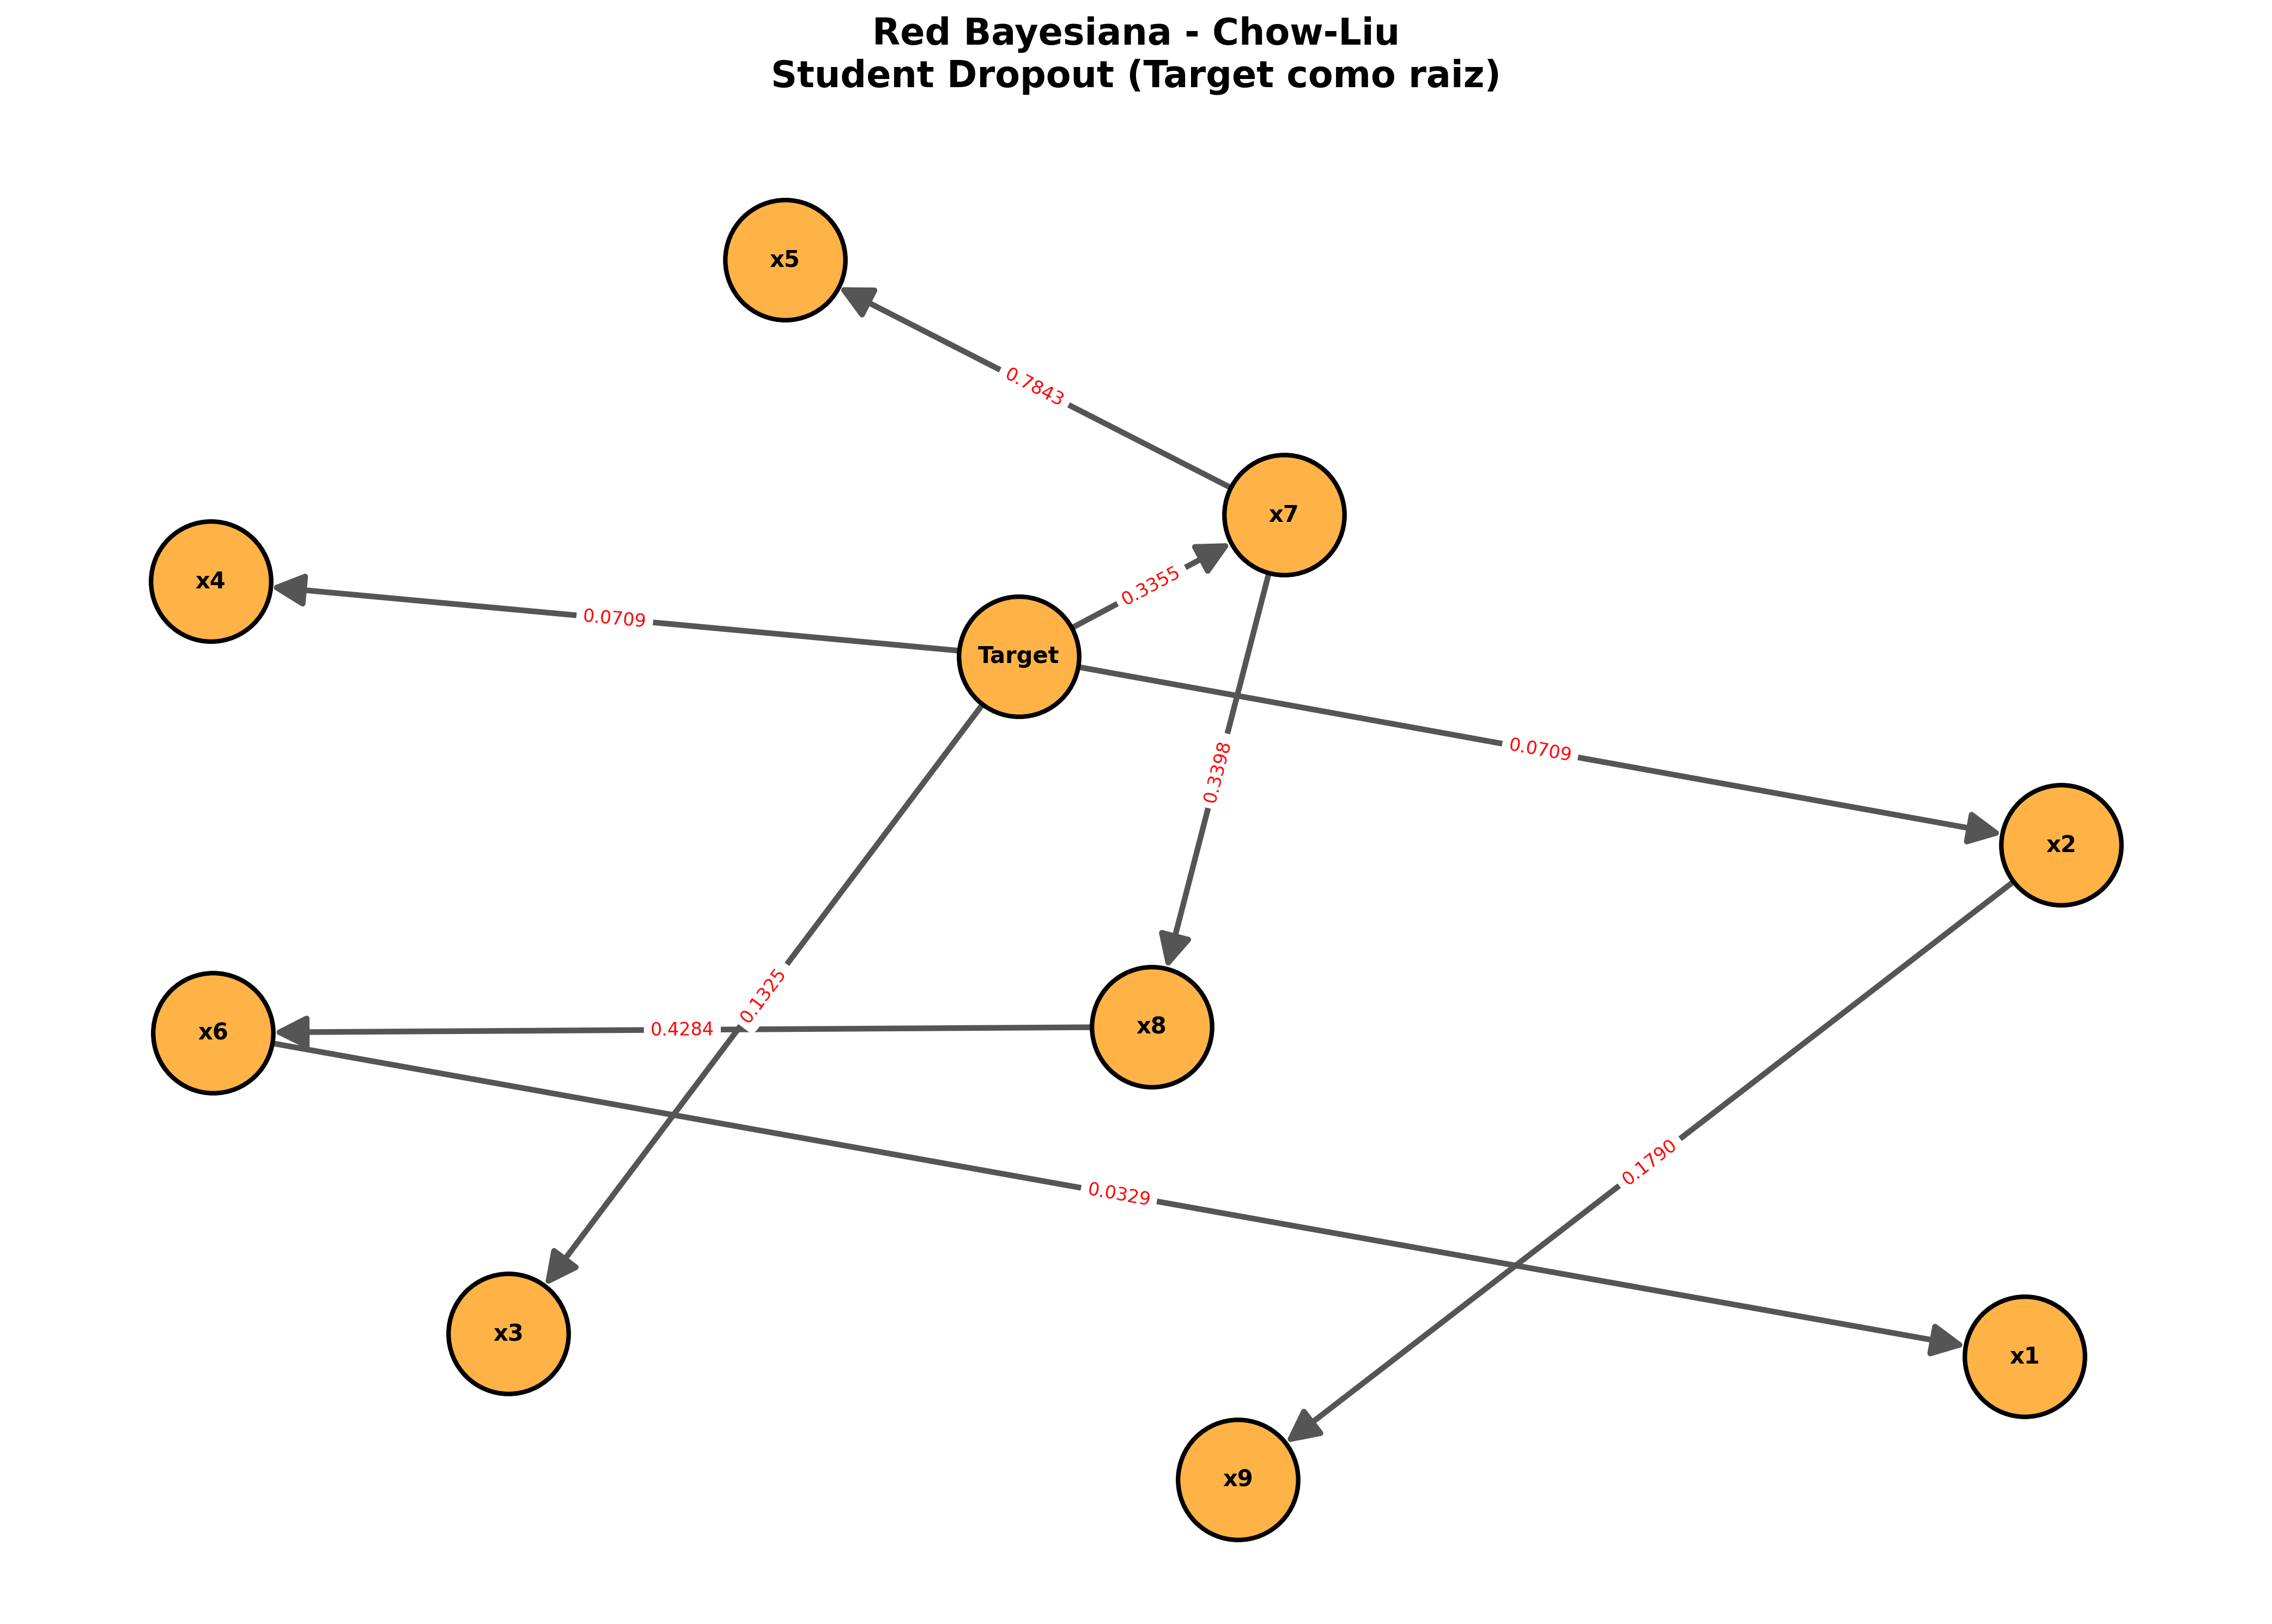
\includegraphics[width=0.85\textwidth]{red_bayesiana.png}
    \caption{Red Bayesiana aprendida mediante Chow-Liu. Target como nodo raíz. Las aristas están dirigidas desde Target hacia las hojas.}
    \label{fig:bayes}
\end{figure}

La estructura dirigida obtenida (usando el dataset original con 4,424 registros) es:

\begin{table}[H]
    \centering
    \begin{tabular}{lll}
        \toprule
        \textbf{Arco} & \textbf{Variable hija} & \textbf{Peso MI} \\
        \midrule
        Target $\rightarrow$ $x_7$ & Aprobados 2do semestre & 0.3355 \\
        Target $\rightarrow$ $x_3$ & Pagos al día & 0.1325 \\
        Target $\rightarrow$ $x_4$ & Becado & 0.0709 \\
        Target $\rightarrow$ $x_2$ & Edad & 0.0709 \\
        $x_7$ $\rightarrow$ $x_5$ & Aprobados 1er semestre & 0.7843 \\
        $x_7$ $\rightarrow$ $x_8$ & Nota 2do semestre & 0.3398 \\
        $x_8$ $\rightarrow$ $x_6$ & Nota 1er semestre & 0.4284 \\
        $x_6$ $\rightarrow$ $x_1$ & Nota de admisión & 0.0329 \\
        $x_2$ $\rightarrow$ $x_9$ & Estado civil & 0.1790 \\
        \bottomrule
    \end{tabular}
    \caption{Estructura del DAG aprendido (Chow-Liu sobre dataset original).}
\end{table}

\subsection{Tablas de Probabilidad Condicional (CPTs)}

Para los nodos conectados directamente al Target, se calculan las distribuciones de probabilidad condicional. Estas CPTs permiten realizar inferencia en la red.

\subsubsection{CPT: $P(x_7 \mid Target)$}

\begin{table}[H]
    \centering
    \begin{tabular}{c|ccc}
        \toprule
        \textbf{Target} & $P(x_7=0)$ & $P(x_7=1)$ & $P(x_7=2)$ \\
        \midrule
        Dropout (0) & 0.8220 & 0.1288 & 0.0493 \\
        Enrolled (1) & 0.5756 & 0.3212 & 0.1033 \\
        Graduate (2) & 0.1159 & 0.5672 & 0.3169 \\
        \bottomrule
    \end{tabular}
    \caption{Probabilidad condicional de aprobados en 2do semestre dado el Target.}
\end{table}

Interpretación: Si un estudiante abandona (Dropout), hay un $82.2\%$ de probabilidad de que tenga bajo rendimiento ($x_7 = 0$) en el segundo semestre. Si se gradúa, solo un $11.6\%$ tiene bajo rendimiento.

\subsubsection{CPT: $P(x_3 \mid Target)$}

\begin{table}[H]
    \centering
    \begin{tabular}{c|cc}
        \toprule
        \textbf{Target} & $P(x_3=0)$ & $P(x_3=1)$ \\
        \midrule
        Dropout (0) & 0.3216 & 0.6784 \\
        Enrolled (1) & 0.0529 & 0.9471 \\
        Graduate (2) & 0.0131 & 0.9869 \\
        \bottomrule
    \end{tabular}
    \caption{Probabilidad condicional de pagos al día dado el Target.}
\end{table}

Interpretación: Los estudiantes que abandonan tienen un $32.2\%$ de probabilidad de no tener los pagos al día, frente a solo $1.3\%$ de los graduados.

\subsection{Ejemplo de Inferencia}

Utilizando las CPTs y la estructura del DAG, es posible realizar inferencia probabilística. A continuación se presenta un ejemplo de inferencia directa desde los datos:

\textbf{Pregunta:} ¿Cuál es la probabilidad de abandono para un estudiante con baja nota de admisión ($x_1 = 0$) y que no tiene los pagos al día ($x_3 = 0$)?

\begin{align*}
    P(Target = Dropout \mid x_1 = 0, x_3 = 0) &= 0.9207 \quad (92.1\%) \\
    P(Target = Enrolled \mid x_1 = 0, x_3 = 0) &= 0.0573 \quad (5.7\%) \\
    P(Target = Graduate \mid x_1 = 0, x_3 = 0) &= 0.0220 \quad (2.2\%)
\end{align*}

Este resultado muestra que la combinación de baja nota de admisión y falta de pago es un predictor extremadamente fuerte de abandono universitario: más del $92\%$ de los estudiantes con este perfil terminan abandonando.

\subsection{Conclusiones de la Red Bayesiana}

\begin{itemize}
    \item El algoritmo de Chow-Liu proporciona una estructura de red Bayesiana que es \textbf{exactamente el MST} calculado en las secciones anteriores, validando la coherencia entre ambos enfoques.
    \item La orientación desde Target como raíz revela una \textbf{jerarquía natural}: el Target influye directamente sobre variables financieras ($x_3$, $x_4$) y de rendimiento ($x_7$), que a su vez influyen sobre otras variables académicas en cascada.
    \item Las CPTs permiten \textbf{cuantificar el riesgo} de abandono para perfiles específicos de estudiantes, lo cual tiene aplicaciones prácticas en sistemas de alerta temprana.
    \item La red Bayesiana obtenida es un modelo \textbf{explicable e interpretable}, donde cada arco tiene un significado causal plausible en el contexto educativo.
\end{itemize}

% =============================================
% ANEXOS
% =============================================
\newpage
\section{Anexos: Código Fuente}

El código fuente completo del proyecto (Python, LaTeX, datos y resultados) está disponible en el repositorio de GitHub:

\begin{center}
    \url{https://github.com/HidenXye/Lenguajes-Split}
\end{center}

El archivo \texttt{resolucion\_dropout.py} implementa: carga y discretización de variables, cálculo de entropía paso a paso, matriz de Información Mutua, construcción del MST mediante los algoritmos de Kruskal y Prim, análisis de sensibilidad rVP con distancias de camino, y aprendizaje de la red Bayesiana mediante el algoritmo de Chow-Liu.

\end{document}
